% SIAM Article Template
\documentclass[review,onefignum,onetabnum]{siamart190516}

% Information that is shared between the article and the supplement
% (title and author information, macros, packages, etc.) goes into
% ex_shared.tex. If there is no supplement, this file can be included
% directly.

%\usepackage{amsmath,amssymb}
\usepackage{mathtools}
\usepackage[T1]{fontenc}     % 8-bit T1 encoding → defines \k, \l, etc.
\usepackage[utf8]{inputenc}  % if your .tex/.bib are UTF-8
\usepackage{lmodern}         % Latin Modern fonts (T1 variants)
\usepackage[hyphens]{url}    % URLs in bib
\usepackage{hyperref}        % clickable links (load after most packages)

% SIAM Shared Information Template
% This is information that is shared between the main document and any
% supplement. If no supplement is required, then this information can
% be included directly in the main document.


% Packages and macros go here
\ifpdf
  \DeclareGraphicsExtensions{.eps,.pdf,.png,.jpg}
\else
  \DeclareGraphicsExtensions{.eps}
\fi

% Add a serial/Oxford comma by default.
\newcommand{\creflastconjunction}{, and~}
\newcommand{\IP}{IP$_3$}
\newcommand{\Ca}{$\textrm{Ca}^{2+}$~}
\newcommand{\R}{\mathbb{R}}
\newcommand{\cc}{$c_c$}
\newcommand{\ce}{$c_e$}
\newcommand{\co}{$c_o$}
\newcommand{\btot}{$b^{tot}$}
\newcommand{\betot}{$b_e^{tot}$}
\newcommand{\Dc}{$D_c$}
\newcommand{\Db}{$D_b$}
\newcommand{\Dce}{$D_{ce}$}
\newcommand{\Dbe}{$D_{be}$}
\newcommand{\ER}{Endoplasmic Reticulum}

% Used for creating new theorem and remark environments
\newsiamremark{remark}{Remark}
\newsiamremark{hypothesis}{Hypothesis}
\crefname{hypothesis}{Hypothesis}{Hypotheses}
\newsiamthm{claim}{Claim}

% Sets running headers as well as PDF title and authors
\headers{A computational study of Alzheimer's disease}{P. Borole, J. M. Rosado, M. Neal, and G. Queisser}

% Title. If the supplement option is on, then "Supplementary Material"
% is automatically inserted before the title.
\title{Neuronal Resilience and Calcium Signaling Pathways in the Context of Synapse Loss and Calcium Leaks: A computational modelling study and Implications for Alzheimer's Disease\thanks{Submitted to the editors \today}}
%\funding{This work was funded by the Fog Research Institute under contract no.~FRI-454.}}}

% Authors: full names plus addresses.
\author{
Piyush Borole\thanks{University of Edinburgh, Edinburgh, Scotland, United Kingdom}
\and James M. Rosado\thanks{Department of Mathematics, Temple University, Philadelphia, Pennsylvania, U.S.A.}
\and MeiRose Neal\footnotemark[3]
 \and Gillian Queisser\footnotemark[3] 
}
\usepackage{amsopn}
\DeclareMathOperator{\diag}{diag}

%%% Local Variables: 
%%% mode:latex
%%% TeX-master: "ex_article"
%%% End: 


% Optional PDF information
\ifpdf
\hypersetup{
  pdftitle={A computational study of Alzheimer's disease},
  pdfauthor={P. Borole, J. M. Rosado, M. Neal, and G. Queisser}
}
\fi

% The next statement enables references to information in the
% supplement. See the xr-hyperref package for details.

%%%%%
\usepackage{xr}
\makeatletter

\newcommand*{\addFileDependency}[1]{% argument=file name and extension
\typeout{(#1)}% latexmk will find this if $recorder=0
% however, in that case, it will ignore #1 if it is a .aux or 
% .pdf file etc and it exists! If it doesn't exist, it will appear 
% in the list of dependents regardless)
%
% Write the following if you want it to appear in \listfiles 
% --- although not really necessary and latexmk doesn't use this
%
\@addtofilelist{#1}
%
% latexmk will find this message if #1 doesn't exist (yet)
\IfFileExists{#1}{}{\typeout{No file #1.}}
}
\makeatother

\newcommand*{\myexternaldocument}[1]{%
\externaldocument[nocite]{#1}%
\addFileDependency{#1.tex}%
\addFileDependency{#1.aux}%
}
%------------End of helper code--------------

% put all the external documents here!
\myexternaldocument{ex_supplement}
%%%%

% FundRef data to be entered by SIAM
%<funding-group specific-use="FundRef">
%<award-group>
%<funding-source>
%<named-content content-type="funder-name"> 
%</named-content> 
%<named-content content-type="funder-identifier"> 
%</named-content>
%</funding-source>
%<award-id> </award-id>
%</award-group>
%</funding-group>

% ORCID Q:0000-0003-4691-5276
\begin{document}

\maketitle

% REQUIRED
\begin{abstract}
In this paper a coupled electro-calcium model was developed and implemented to computationally explore the effects of neuronal synapse loss, in particular in the context of Alzheimer's disease. Established parameters affected by Alzheimer's disease, such as synapse loss, calcium leaks at deteriorating synaptic contacts, and downregulation of the calcium-buffer Calbindin, are subject to this study. Reconstructed neurons are used to define the computational domain for a system of partial and ordinary differential equations, discretized by finite differences and solved with a semi-implicit second order time integrator. The results show neuronal resilience during synapse loss. When incorporating calcium leaks at affected synapses, neurons lose their ability to produce synapse to nucleus calcium signals, necessary for learning, plasticity, and neuronal survival. Downregulation of Calbindin concentrations partially recovers the signaling pathway to the cell nucleus. These results could define future research pathways towards stabilizing the calcium signaling pathways during Alzheimer's disease. The coupled electro-calcium model was implemented and solved using Matlab.
\end{abstract}

% REQUIRED
\begin{keywords}
  Multiscale Modeling, Neurons, Calcium, Dendrites, Synapse Loss, Amyloid $\beta$, Hodgkin-Huxley, Plasticity, Numerical Analysis, Alzheimer's Disease
\end{keywords}

% Multiscale Modeling, Numerical Analysis, electro-calcium model, Synapse Loss, Amyloid $\beta$, Alzheimer's Disease
% Gillian Queisser
% Department of Mathematics
% Temple University
% 1805 N Broad Street
% Philadelphia, PA 19122-6094, USA
% https://math.temple.edu/~queisser/
% phone: +1 (267) 294-1428
% REQUIRED
\begin{AMS}
  92-10, 00A69, 65K05, 92C20
\end{AMS}


%**************************************************************************%
%NEW SECTION$
%**************************************************************************%

\section{Introduction}
Degeneration of neuronal signaling due to ageing and neuropathologies, such as Alzheimer's and Parkinson's disease \cite{marambaud2009calcium, berridge2003calcium, berridge1998neuronal,  mattson2007calcium, green2008linking, alberdi2010amyloid, carafoli1975role, demuro2010calcium, itkin2011calcium, surmeier2007calcium, calbi2001condensed}, has become a very important research area. During ageing, or due to pathologies, changes in synaptic information transfer and intracellular responses to neuronal network communication disrupt the finely regulated intracellular signaling cascades, that enable neurons to control gene transcription responses \cite{berridge1998neuronal,di2009decoding}. These responses have been shown to affect learning, cellular plasticity, neuronal health, and cell survival \cite{berridge2003calcium,lohmann2005regulation,michaelsen2010calcium,redmond2005regulation}. Intracellular calcium signaling has been shown to play an outsized role in regulating information transfer from synaptic sites to the cell nucleus \cite{hagenston2011calcium, hardingham2004synapse, greer2008synapse, deisseroth2003signaling}, which harbors the DNA. Disruption of calcium signals, induced by neurodegenerative diseases, is implicated in neuronal decay and onset of clinical symptoms \cite{kawahara2004disruption, pollard1993new}. Taking Alzheimer's disease (AD) as an example, accumulation of amyloid-$\beta$ proteins at chemical synapses disrupts synaptic communication \cite{spires2014intersection,tu2014oligomeric,shankar2009alzheimer,karisetty2020amyloid,marsh2018synaptic}, as well as the intracellular calcium machinery. Calcium leaks \cite{demuro2010calcium,itkin2011calcium,demuro2011single, lin1999amyloid, kawahara1997alzheimer, quist2005amyloid,di2014interaction,di2016common,lal2007amyloid}, changes in ryanodine-receptor (RyR) activity, which causes increased calcium release from the endoplasmic reticulum (ER) into the cytosol \cite{shtifman2010amyloid}, as well as reduction of the calcium-buffering molecule calbindin \cite{iacopino1990specific, kook2014crucial, crapper1987calmodulin, palop2003neuronal}, are all consequences of Alzheimer-induced degeneration.


Since systematic experimental modifications of the calcium machinery, e.g., local changes in the RyR density, the morphology of the ER, or synaptic activation patterns, are extremely hard, if not impossible, to carry out, we decided to develop a computational model that couples an electrical model for ion channel dynamics on the neuronal plasma membrane (PM) with a detailed calcium model that describes the intracellular calcium dynamics governed by PM-exchange mechanisms, store release and sequestration from the ER, and diffusion-reaction processes in the cytosol. Using this model, we then studied calcium dynamics in unmodified, healthy, neurons and compared these to neuropathological states, defined by synapse loss, calcium leaks in the PM, changes in ER refilling, and buffering (cytosolic and ER) capacities.

\textcolor{red}{The focus of this study was to understand the impact of AD pathologies on \Ca signaling in neurons. Previously, calcium models have been used to study parameters associated with stable and abortive \Ca waves \cite{Breit2018,Queisser2018,Rosadoplos2022} in neuronal sub-compartments. Models using full neuron geometries have been used to study electrical dynamics and action potential generation \cite{smith2013dendritic,timofeeva2006dendritic}. Repeated synaptic events need to translate into rapid \Ca release from the ER into the cytosol to initiate stable \Ca signals. This, in turn, requires rapid ER refilling mechanisms. One such mechanism is governed by store-operated-calcium-channels (SOC), which support ER refilling. SOC models have been developed in \cite{mcivor2018three,gil2021three}. Additionally, the ER lumen stores vast amounts of \Ca in buffered form. Buffering dynamics in the ER have been modeled in \cite{higgins2006buffering}. Calcium leaks associated with amyloid-$\beta$ have been studied in \cite{latulippe2018mathematical,de2013progression}. As described previously, another pathology associated with AD is synapse loss which has been studied using neuronal network models \cite{kashyap2019synapse,swietlik2019computer}. Dave et al. \cite{dave2021mathematical} implemented a 3D calcium model and tested the impact of \Ca buffer concentrations on \Ca signaling.
While these models address individual calcium-regulators, we here developed an integrated electro-calcium model to simulate full-cell dynamics from synapse to cell nucleus.}

The biophysical model is solved numerically on computational domains, using detailed morphological reconstructions, available on NeuroMorpho.org \cite{Ascoli2007}. To efficiently solve the bidirectionally coupled electro-calcium model, we discretize the computational domain using finite differences and use the multistep implicit-explicit (ImEx) method known as SBDF2 (second order semi-implicit backward differentiation), \cite{Seibold2019-df,Albi2021} as a time-integrator. We implement a dimensionally reduced set of model equations by way of rotational symmetry of the dendritic branches.

The paper is organized as follows: In Sec. \ref{sec:model} we derive the calcium model, consisting of all relevant calcium-exchange mechanisms, and couple this model to a Hodgkin-Huxley electrical model through voltage-dependent calcium channels (VDCCs). We then detail the process of integrating reconstructed neuron geometries into our numerical simulations, as well as the numerical methods. Is Sec. \ref{sec:experiments} we detail the results from systematically changing parameters relevant in neurodegeneration, followed by a discussion in Sec. \ref{sec:discussion}.

Using our computational framework we were able to show that neurons are capable of generating calcium waves towards the nucleus even under conditions of synapse loss, as seen during AD. Here, lost synapses are classified as no longer active in producing a postsynaptic calcium influx. If, however, those sites become leaky for calcium, a previously reported phenomenon \cite{demuro2010calcium,itkin2011calcium,demuro2011single, lin1999amyloid, kawahara1997alzheimer, quist2005amyloid,di2014interaction,di2016common,lal2007amyloid}, calcium communication between synapses and soma breaks down if the neuron experiences roughly 50\% synapse loss or more. A reduction in the concentration of the calcium buffering molecule calbindin, an effect of AD \cite{iacopino1990specific, kook2014crucial, crapper1987calmodulin,palop2003neuronal}, counters the effect of leaky (and lost) synapses to a certain degree. Based on the presented work it appears that neurons are equipped to compensate a substantial loss of synapses with respect to synapse to nucleus communication. It is the leakiness of deteriorating synapses that causes a collapse of robust calcium signaling. 


%**************************************************************************%
%NEW SECTION$
%**************************************************************************%

\section{The Biophysical Model and Numerical Methods}\label{sec:model}
In this section we derive and describe all model equations, cell geometry integration, and numerical methods for solving the coupled electro-calcium model.

%\iffalse
\subsection{Model Equations}
In this section we discuss the model equations that are used to describe intracellular ion signaling and plasma membrane electrical signal propagation.
The spatio-temporal ion dynamics are modeled by a system of diffusion-reaction equations, found in \cite{Breit2018,Queisser2018}, and are of the form
\begin{equation}
\frac{\partial u}{\partial t} = D\Delta u + R(u), 
\end{equation}
which were adapted for 1D neuronal geometries, by assuming rotational symmetry. Here, $u$ denotes ion concentration, $D$ the corresponding diffusion coefficient, and $R(u)$ a reaction term. We used the Hodgkin-Huxley model (HH) equations \cite{Grein2014,Hodgkin1952C,Hodgkin1952B,Hodgkin1952D,Hodgkin1952A,Hodgkin1952E} for electrical signal dynamics, with sodium (Na$^+$), potassium (K$^+$), calcium (Ca$^{2+}$), and leak ion channel dynamics. We coupled the electrical dynamics with spatio-temporal ions dynamics by including voltage dependent calcium channels (VDCCs) on the plasma membrane. A \textit{feed forward} coupling, in which the membrane potential drives the release of calcium into the cytosol, and a \textit{feed backward} coupling by including a current flux \cite{koch1989methods} in the HH-model equations which is driven by changes in the cytosolic Ca$^{2+}$ completes bidirectionality of the system.   
%\fi


%***************************************************%
\subsection{Calcium Dynamics and Membrane Transport Mechanisms} \label{sec:calcium-dynamics-membrane-transport}
In previous work a three-dimensional model for intracellular $\textrm{Ca}^{2+}$ dynamics was derived for the subcellular level \textcolor{black}{\cite{Breit2018,Queisser2018,rosado2022}}. These models, however, were derived to incorporate the detailed three-dimensional architecture of organelles and the cellular plasma membrane and did not include mechanisms of rapid endoplasmic refilling nor Alzheimer-relevant processes. Here, we provide the membrane transport mechanisms and a dimension-reduced one-dimensional model of the original 3D model by assuming local rotation symmetry and uniformly distributed transport mechanisms. The dimension-reduced diffusion-reaction system reads \textcolor{red}{(see supplemental material SM1 for a derivation)}:
\begin{align}
    \frac{\partial c_c}{\partial t}&=\frac{1}{(R^2-r^2)}\frac{\partial}{\partial x}\left((R^2-r^2)D_c\frac{\partial c_c}{\partial x}\right)+\left(k_b^-(b^{tot}-b)-k_b^+bc_c\right) \label{eqn:diffcc} \\
    &+\frac{2r}{(R^2-r^2)}J_{ERM}+\frac{2R}{(R^2-r^2)}J_{PM}, \quad \text{in $\Omega_{C}$} \notag \\ \notag \\ 
    \frac{\partial c_e}{\partial t}&=\frac{1}{r^2}\frac{\partial}{\partial x}\left(r^2D_c\frac{\partial c_e}{\partial x}\right) + \left(k_{be}^-(b_e^{tot}-b_e)-k_{be}^+b_ec_e\right) \label{eqn:diffce} \\ \notag \\
    & -\frac{2}{r}J_{ERM} + \frac{2}{r}J_{SOC}, \quad \text{in $\Omega_{ER}$} \notag \\ \notag \\
    \frac{\partial b}{\partial t}&=\frac{1}{(R^2-r^2)}\frac{\partial}{\partial x}\left((R^2-r^2)D_b\frac{\partial b}{\partial x}\right)+\left(k_b^-(b^{tot}-b)-k_b^+bc_c\right), \quad \text{in $\Omega_{C}$}\label{eqn:diffb}\\  \notag \\
    \frac{\partial b_e}{\partial t}&=\frac{1}{r^2}\frac{\partial}{\partial x}\left(r^2D_{be}\frac{\partial b_e}{\partial x}\right)+\left(k_{be}^-(b_e^{tot}-b_e)-k_{be}^+b_ec_e\right) \quad \text{in $\Omega_{ER}$}\label{eqn:diffbe}%\\  \notag \\
    %\frac{dp}{dt}&=\frac{1}{(R^2-r^2)}\frac{\partial}{\partial x}\left((R^2-r^2)D_p\frac{\partial p}{\partial x}\right)-k_p(p-p^r). \label{eqn:diffp}
\end{align}
Here $R$ is the dendritic radius, $r$ the endoplasmic radius (both are functions of $x$), $k_s^p$ are rate functions controlling chemical reactions, $b_s^{tot}$ the total buffer concentrations in cytoplasm and ER, and $D_s$ are diffusion coefficients. These equations are defined in cytosolic ($\Omega_C$) and ER domains ($\Omega_{ER}$).
Equation \cref{eqn:diffcc} models the diffusion-reaction of cytosolic calcium, where $c_c$ is the cytosolic Ca$^{2+}$ concentration and equation \cref{eqn:diffce} models the diffusion-reaction of ER calcium where $c_e$ is the endoplasmic Ca$^{2+}$ concentration. Equations \cref{eqn:diffb} and \cref{eqn:diffbe} model the diffusion-reaction of cytosolic Calbindin and Calreticulin, where $b$ and $b_e$ are Calbindin and Calreticulin concentrations, respectively. Both molecules buffer calcium, based on the reaction equations
\begin{equation*}
    \textrm{Ca}^{2+}+\textrm{CalB}\xrightleftharpoons[\kappa_b^+]{\kappa_b^-} \textrm{CalB}\textrm{Ca}^{2+},~
    \textrm{Ca}^{2+}+\textrm{CalR}\xrightleftharpoons[\kappa_{be}^+]{\kappa_{be}^-} \textrm{CalR}\textrm{Ca}^{2+}.
\end{equation*}
 The reactions are included in \cref{eqn:diffcc} and \cref{eqn:diffb}, as well as in \cref{eqn:diffce} and \cref{eqn:diffbe}, respectively. Equations \cref{eqn:diffcc}, \cref{eqn:diffce} both contain flux terms corresponding to the $\textrm{Ca}^{2+}$ influx/efflux due to different membrane transport mechanisms (see below). %Equation \cref{eqn:diffp} models the diffusion-reaction of cytosolic IP3 molecules, where $p=[\textrm{IP3}]$ is the concentration of IP3 molecules.
The membrane transport mechanisms are realized by including fluxes $J_{PM}$ and $J_{ER}$. The term $J_{PM}$ is the net $\textrm{Ca}^{2+}$ ion flux across the plasma membrane, and $J_{ERM}$ is the net $\textrm{Ca}^{2+}$ ion flux across the ER membrane. The two fluxes are further compartmentalized by the mechanisms that are transporting $\textrm{Ca}^{2+}$ across the membranes, that is
\begin{align}
    J_{PM} &= -J_P-J_N+J_{VDC}+J_{SYN}+J_{l,p},\quad \text{on $\Gamma_{PM}$} \label{eqnPM} \\
    J_{ERM} &= J_{RyR}-J_S+J_{SOC}+J_{l,e}\label{eqnER} \quad \text{on $\Gamma_{ERM}$}.
\end{align}
The flux terms for the plasma membrane ($\Gamma_{PM}$) are as follows: $J_P$ is the $\textrm{Ca}^{2+}$ flux from plasma membrane $\textrm{Ca}^{2+}$-ATPase pumps (PMCA), $J_N$ is the flux due to $\textrm{Na}^+/\textrm{Ca}^{2+}$ exchangers (NCX), $J_{VDC}$ is the flux from VDCCs, $J_{SYN}$ is the calcium influx through the post-synaptic density (PSD), and $J_{l,p}$ is the leak calcium flux across the plasma membrane. 

Fig.~\ref{fig:Illustration}A provides an overview of various components and their operating domains modeled in this study in an unbranched neurite. Fig.~\ref{fig:Illustration}B,C provides a visualization of the full neuron geometry used in this study in 2D and 3D view. 

The flux terms for the ER are as follows: $J_{SOC}$ is the flux from store-operated calcium channels \cite{mcivor2018three,gil2021three}, $J_{RyR}$ is the flux from to ryanodine receptors \cite{Queisser2018,Breit2018,Keizer1996,Rosadoplos2022,rosado2022}, $J_S$ is the flux from sarco/endoplasmic reticulum $\textrm{Ca}^{2+}$-ATPase pumps \cite{Sneyd2003}, and $J_{l,e}$ is the leak calcium flux. Each flux term is of the form
\begin{align}
J_X = \rho_X\cdot p_X^o\cdot I_X, \label{eqnFlux}
\end{align} 
where $\rho_X$ is the density of the transport mechanism per unit area, $p_X^o$ is the open state probability of a single channel which is unitless, and $I_X$ is the $\textrm{Ca}^{2+}$ current in units of concentration per time. Homogeneous distributions of all exchange mechanisms were assumed, as experimental data on precise numbers of spatial distribution of these mechanisms are not readily available. In the following paragraphs we describe each of the flux functions used in our study, along with references to the published models and available experimental data.

\begin{figure}[!ht]
    \centering
    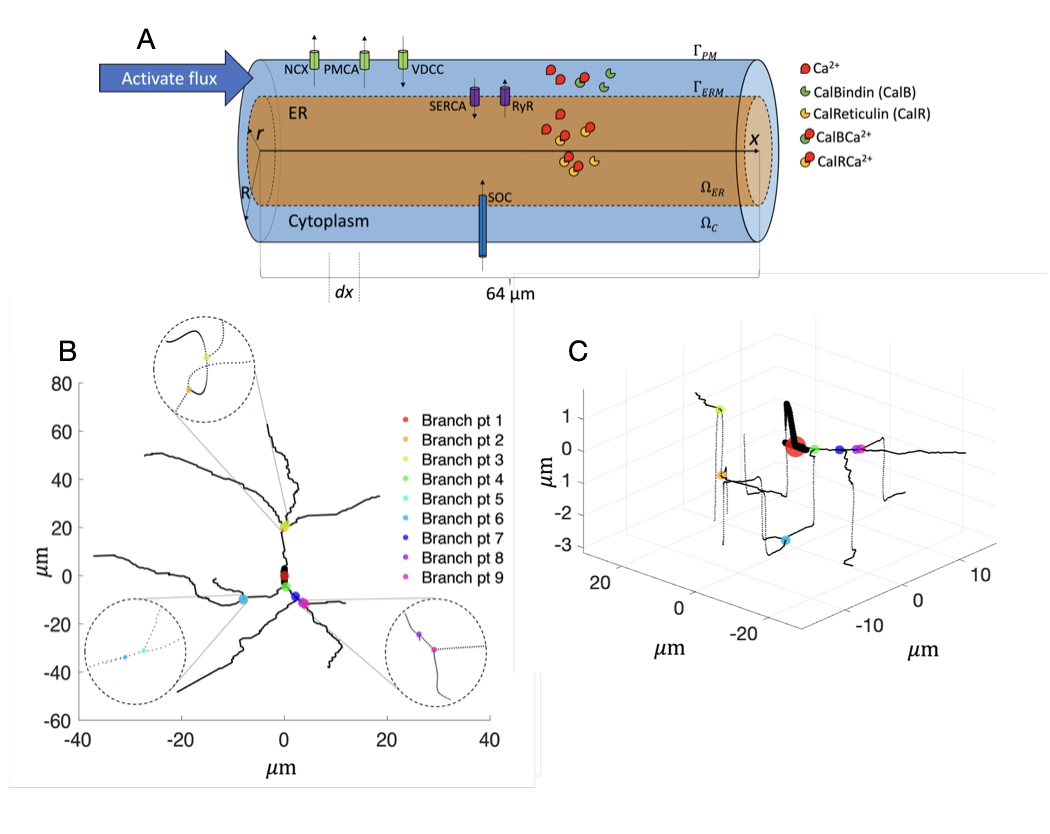
\includegraphics[width=12cm]{Figures/illustrationJuly14_2023.png}
    \caption{(A) Schematic of unbranched neurite with model components and simulation domains. The neurite is 64 $\mu m$ in length with dendrite radius ($R = 0.4~\mu m$) and ER radius ($r = 0.15~\mu m$). The two domains are ER ($\Omega_{ER}$) and cytoplasm ($\Omega_{C}$) with $\Gamma_{PM}$ and $\Gamma_{ERM}$ being plasma membrane (PM) and ER membrane (ERM) boundary. $\textrm{Ca}^{2+}$ is present in both cytoplasm and ER domains while Calbindin and Calreticulin are present only in cytoplasm and ER, respectively. The $\textrm{Ca}^{2+}$ buffering reaction and diffusion takes places in $\Omega_{ER}$ and $\Omega_{C}$ domains. NCX, PMCA and VDCC transports $\textrm{Ca}^{2+}$ across PM. SERCA and RyR transports $\textrm{Ca}^{2+}$ across ERM. For our simulation settings, SOC transports $\textrm{Ca}^{2+}$ from extracellular space to ER. Activation flux enters through cytoplasmic domain on the left hand side. (B) Full neuron geometry used in the presented simulations with $9$ branching points. (C) 3D view of the geometry with branching points. The thick region at the branching point 1 (red point) is the soma of the neuron} 
    \label{fig:Illustration}
\end{figure}

\textit{\textbf{PMCA Pumps.}} For the PMCA pumps we used the model found in \cite{Graupner2005,Graupner2003}, where the plasma membrane $\textrm{Ca}^{2+}$ current is modeled as a second-order Hill equation
\[
J_P(c_c)=\rho_P\cdot\frac{I_P c_c^2}{K_P^2+c_c^2},
\]
where $\rho_P$ is the density of PMCA pumps on the plasma membrane, $I_P$ is the single channel $\textrm{Ca}^{2+}$ current, $c_c$ is the cytosolic $\textrm{Ca}^{2+}$ concentration, and $K_P$ is the measure of $\textrm{Ca}^{2+}$ affinity. Values for the constants in this equation were borrowed from \cite{Breit2018,Queisser2018}.

\textit{\textbf{NCX Exchangers.}} The NCX exchange mechanism moves $\textrm{Ca}^{2+}$ from the cytosol to the extracellular region of the neuron. The NCX transport mechanism is responsible for keeping the cytosolic calcium concentration low, and has low affinity to calcium, i.e. the NCX proteins do not bind closely to calcium ions. Therefore, in order for NCX pumps to be effective, they need to register high calcium concentrations. For the NCX exchange current we assume a fixed $\textrm{Na}^+$ concentration at the plasma membrane, utilizing a first-order Hill equation from \cite{Graupner2005,Graupner2003}:
\[
J_N(c_c)=\rho_N\cdot\frac{I_Nc_c}{K_N+c_c},
\]
where $\rho_N$ is the density of NCX exchangers on the plasma membrane, $I_N$ is the single channel $\textrm{Ca}^{2+}$ current, $c_c$ is the cytosolic $\textrm{Ca}^{2+}$ concentration, and $K_N$ is the measure of $\textrm{Ca}^{2+}$ affinity for NCX exchangers. All values for the constants in this equation were borrowed from \cite{Breit2018,Queisser2018}.

\textit{\textbf{VDCCs.}} For the voltage dependent calcium channels, we follow the Borg-Graham model found in \cite{Grein2014,BorgGraham1999} and the $\textrm{Ca}^{2+}$ current is given by 
\[
J_{VDC}(V,c_c,t) = G(V,t)F(V,\Delta[\textrm{Ca}^{2+}]),
\]
where $G(V,t)\in [0,1]$ is the gating function which depends on the membrane voltage $V$ at time $t$, and $F(\cdot,\cdot)$ is the flux function. Both of these functions depend on the voltage at the channel at time $t$ and we assume a prescribed density on the plasma membrane. For the flux function $F(\cdot,\cdot)$, the quantity $\Delta [\textrm{Ca}^{2+}]$ is the difference between the cytoplasmic and extracellular ($c_o$) ion concentration
\[
\Delta [\textrm{Ca}^{2+}] = c_c-c_o
\]
and the flux function is computed using the Goldman-Hodgkin-Katz equation
\[
F\left(V, \Delta [\textrm{Ca}^{2+}]\right) = \bar{p}_{\textrm{Ca}^{2+}}\frac{Vz^2 F^2}{RT}\cdot\frac{c_c-c_o \exp(-zFV/RT)}{1-\exp (-zFV/RT)},
\]
where $R$ is the universal gas constant, $F$ is Faraday's constant, $T$ is temperature in Kelvin, $\bar{p}_{\textrm{Ca}^{2+}}$ is the permeability of $\textrm{Ca}^{2+}$ ions through the channels, and $z$ is the valence of a $\textrm{Ca}^{2+}$ ion. The gating function is expressed as
\[
G(V,t)  =\prod_{i} x_i^{n_i}(V,t), 
\]
where $x_i^{n_i}$ is the open probability of the $\textrm{Ca}^{2+}$ gating particle and $n_i$ is the number of particles. The open probability is described by the ODE
\[
\frac{dx_i}{dt} = \frac{x_\infty(V)-x_i}{\tau_{x_i}(V)},
\]
where $x_\infty$ is the steady-state value of the probability, and $\tau_{x_i}$ is the time constant for the particular particle. Each particle has an associated kinetic function for the open and closed states, in this case it is $\alpha_i(V)$ and $\beta_i(V)$, and from this we compute the time constant
\[
\tau_{x_i} = \frac{1}{\alpha_i'(V)+\beta_i'(V)}+\tau_0.
\]
As an example, the gating function $G(\cdot)$ for N-Type VDCCs is described by
\[
G(V,t)=k(V,t)l^2(V,t),
\] 
where the gating functions $k(\cdot)$ and $l(\cdot)$ satisfy the ODEs
\begin{align*}
\frac{\partial k}{\partial t}&=\frac{k_{\infty}-k}{\tau_k}\ \ \ \textrm{and}\ \ \ \frac{\partial l}{\partial t}=\frac{l_{\infty}-l}{\tau_l},
\end{align*}
where
\[
k_{\infty}=\frac{\alpha_k(V)}{\alpha_k(V)+\beta_k(V)};\ \ \ l_{\infty}=\frac{\alpha_l(V)}{\alpha_l(V)+\beta_l(V)},
\]
and
\[
\tau_k = \frac{1}{\alpha_k+\beta_k}+\tau_{k,0}; \ \ \ 
\tau_l = \frac{1}{\alpha_l+\beta_l}+\tau_{l,0}.
\]
The rate functions are given by
\begin{align*}
\alpha_k(V)&=K_k\exp\left(\frac{z_k\gamma_k\left(V-V_{1/2,k}\right)F}{RT}\right)\\
\beta_k(V)&=K_k\exp\left(\frac{-z_k(1-\gamma_k)\left(V-V_{1/2,k}\right)F}{RT}\right)\\
\alpha_l(V)&=K_l\exp\left(\frac{z_l\gamma_l\left(V-V_{1/2,l}\right)F}{RT}\right)\\
\beta_l(V)&=K_l\exp\left(\frac{-z_l(1-\gamma_l)\left(V-V_{1/2,l}\right)F}{RT}\right)
\end{align*}
and the values and descriptions of the constants used in the above equations can be found in \cite{Grein2014}.

Additionally, we also utilize parameters found in \cite{BorgGraham1999, Grein2014} that differentiate between N-type and T-type channels which are high-voltage-activate (HVA) and low-voltage-activated (LVA), respectively.

For the presented research we compared the cytoplasmic \Ca response for a model with and without VDCC coupling. For VDCC coupling, we tested N-type and T-type channels, using parameters found in \cite{BorgGraham1999, Grein2014}. We noticed that the coupled VDCC models have different cytoplasmic \Ca responses compared to the uncoupled VDCC model (see supplemental Fig. SM3).  


\textit{\textbf{RyR Channels.}} The model equations for ryanodine receptor (RyR) channels are of the form
\[
J_{RyR}(c_c,c_e) = \rho_{RyR}\cdot p_{RyR}^o\cdot I_{RyR}(c_c,c_e),
\]
where $\rho_{RyR}$ is the density, $p_{RyR}^o$ is the open state probability, and $I_{RyR}(c_c,c_e)$ is the $\textrm{Ca}^{2+}$ current through a single RyR channel. From \cite{Queisser2018,Breit2018,Keizer1996,Rosadoplos2022,rosado2022} we describe the current by
\[
I_{RyR}(c_c,c_e)=I_{RyR}^{ref}\cdot\frac{c_e-c_c}{c_e^{ref}},
\]
where the reference current $I_{RyR}^{ref}$ is taken from data found in \cite{Tinker1993}. The open probability for RyR channels is taken from \cite{Queisser2018,Breit2018,Keizer1996}, which is calculated by summing the two open states $o_1$ and $o_2$, that is $ p_{RyR}^o=o_1+o_2$. The values of the open states are governed by a system of ordinary differential equations
\begin{align*}
    o_1 &= 1- c_1-o_2-c_2,\\
    \frac{\partial c_1}{\partial t} &= k_a^-o_1-k_a^+c_c^4c_1,\\
    \frac{\partial o_2}{\partial t} &= k_b^+c_c^3o_1-k_b^-o_2,\\
    \frac{\partial c_2}{\partial t} &= k_c^+o_1-k_c^-c_2,
\end{align*}
where the kinetic values $k_a^\pm$, $k_b^\pm$, and $k_c^\pm$ are given in Table SM1. This system of ODEs is solved independently at every point on the 1D domain of the ER.


\textit{\textbf{SERCA Pumps.}} For the current flux from sarco/endoplasmic reticulum $\textrm{Ca}^{2+}$-ATPase (SERCA) pumps we use a model from \cite{Sneyd2003} given by
\[
J_S(c_c,c_e) = \rho_S\cdot\frac{I_Sc_c}{(K_S+c_c)c_e},
\]
where $\rho_S$ is the density of SERCA pumps on the ER membrane, $I_S$ is the maximum $\textrm{Ca}^{2+}$ current, and $K_S$ is the affinity of $\textrm{Ca}^{2+}$. This model was chosen because it includes the dependence of $\textrm{Ca}^{2+}$ current on the cytoslic $\textrm{Ca}^{2+}$ concentration and ER saturation. The values of the constants are given in Table SM1.

\iffalse
\begin{table}[htbp]
{%\footnotesize
  \fontsize{6.5pt}{8.0pt}\selectfont
  \caption{Model Parameters}  \label{tab:modelparameters}
\begin{center}
  \begin{tabular}{|cccc|} \hline
   \bf Parameter & \bf Symbol & \bf Value & \bf Reference \\ \hline
    & \multicolumn{2}{c}{\textit{Initial and equilibrium values}}   &  \\
    Cytosolic \Ca &  \cc & $50~ nM$ & \cite{Queisser2018}\\
    ER \Ca & \ce & $250~ \mu M$ & \cite{Queisser2018}\\
    Reference ER \Ca & $c_e^{ref}$ & $250~ \mu M$ & \cite{Queisser2018}\\
    Extracellular \Ca & \co & $1~ mM$ & \cite{Queisser2018} \\
    Total Calbindin D$_{28k}$ (Cytosol) & \btot  & $40~ \mu M$ & \cite{muller2005endogenous,Queisser2018} \\
    Total Calreticulin (ER) & \betot &  $3.6~ mM$ & \cite{means2006reaction} \\
    &  & & \\
    & \multicolumn{2}{c}{\textit{Diffusion/reaction}}  &  \\
    Diffusion coefficient (\cc)  & \Dc & $220~ \mu m^2 s^{-1}$ & \cite{allbritton1992range,Queisser2018} \\
    Diffusion coefficient (CalB)  & \Dc & $20~ \mu m^2 s^{-1}$ & \cite{schmidt2003mutational,Queisser2018} \\
    CalB forward rate & $\kappa_b^+$ & $27~ \mu M^{-1}s^{-1}$ & \cite{muller2005endogenous,Queisser2018}\\
    CalB backward rate & $\kappa_b^-$ & $19~ s^{-1}$ & \cite{muller2005endogenous,Queisser2018}\\
    Diffusion coefficient (\ce)  & \Dce & $10~ \mu m^2 s^{-1}$ & \cite{dayel1999diffusion,mcivor2018three} \\
    Diffusion coefficient (CalR)  & \Dbe & $27~ \mu m^2 s^{-1}$ & \cite{means2006reaction} \\
    CalR forward rate & $\kappa_{be}^+$ & $10^5~ M^{-1}s^{-1}$ & \cite{means2006reaction}\\
    CalR backward rate & $\kappa_{be}^-$ & $200~ s^{-1}$ & Calculated using \\ 
    &  & & $K_d = 2~mM$ (\cite{baksh1991expression})\\
    &  & & \\
    & \multicolumn{2}{c}{\textit{RyR channel}}   & \\
    $o_1 \to c_1$ &  $k_a^-$ & $28.8~ s^{-1}$ & \cite{Keizer1996}\\
    $c_1 \to o_1$ &  $k_a^+$ & $1500~ \mu M^{-4}s^{-1}$ & \cite{Keizer1996}\\
    $o_2 \to o_1$&  $k_b^-$ & $385.9~ s^{-1}$ & \cite{Keizer1996}\\
    $o_1 \to o_2$&  $k_b^+$ & $1500~ \mu M^{-3}s^{-1}$ & \cite{Keizer1996}\\
    $c_2 \to o_1$&  $k_c^-$ & $0.1~ s^{-1}$ & \cite{Keizer1996}\\
    $o_1 \to c_2$&  $k_c^+$ & $1.75~ s^{-1}$ & \cite{Keizer1996}\\
    Reference current & $I_{RyR}^{ref}$ & $3.5 \times 10^{-18}~ mol~s^{-1}$& \cite{Tinker1993}\\ 
    &  & & \\
    & \multicolumn{2}{c}{\textit{SERCA pumps}}   & \\
    SERCA current &  $I_S$ & $6.5 \times 10^{-21}~ mol~\mu M~s^{-1}$ & \cite{chiu1980rapid,Queisser2018}(Adapt.)\\
    & $K_S$  & $180~ nM$ & \cite{Sneyd2003}\\
    SERCA density & $\rho_S$ & $2390~ \mu m^{-2}$ & \cite{means2006reaction}(Approx.)\\
    &  & & \\
    & \multicolumn{2}{c}{\textit{PMCA pumps}} & \\
    PMCA current &  $I_P$ & $1.7 \times 10^{-23}~ mol~s^{-1}$ & \cite{Graupner2003}\\
    Measure of \Ca affinity & $K_P$  & $ 60~ nM$ & \cite{elwess1997plasma}\\
    PMCA density & $\rho_P$ & $500~ \mu m^{-2}$ & \cite{Queisser2018}(Estim.)\\
    &  & & \\
    & \multicolumn{2}{c}{\textit{NCX pumps}} & \\
    NCX current &  $I_N$ & $2.5 \times 10^{-21}~ mol~s^{-1}$ & \cite{Graupner2003}(adapt.)\\
    Measure of \Ca affinity & $K_N$  & $ 1.8~ \mu M$ & \cite{Graupner2003}\\
    NCX density & $\rho_N$ & $15~ \mu m^{-2}$ & \cite{Queisser2018}(Estim.)\\
    &  & & \\
    &  \multicolumn{2}{c}{\textit{Store Operated Channels}} & \\
    Single SOC current &  $I^{ref}_{SOC}$ & $2.1~ fA$ & \cite{gil2021three,hoth1992depletion}\\
    Faraday's Constant & $F$ & $96485~ C/mol$ & \\
    Valency of \Ca ~ion & $z$ & 2 & \\
    Density of SOC & $\rho_{SOC}$ & $0.4 ~\mu m^{-2}$ & choosen\\
    &  & & \\
    &\multicolumn{2}{c}{\textit{A$\beta$ pores}} & \\
    Rate constant & $k_{\beta}$ & $1~ s^{-1}$ & \cite{latulippe2018mathematical,de2013progression}\\
    Cooperative factor & $m$ & $4$ & \cite{latulippe2018mathematical,de2013progression}\\
    Concentration of A$\beta$ & a & $5 ~nM$, $100 ~\mu M$ & \cite{de2013progression,paula2011amyloid}\\
    & & &\\
    %&  \textit{Leakages} & & \\
    %Leakage velocity ERM & $v_{l,e}$ & $~ nm~s^{-1} $ & (Calc.)\\
    %Leakage velocity PM & $v_{l,p}$ & $~ nm~s^{-1} $ & (Calc.) \\
    %& & &\\
    & \multicolumn{2}{c}{\textit{Miscellaneous}} & \\
    Input synaptic flux & $j_{syn}$ & $1 \times 10^{-6}~ $ & \cite{Queisser2018,rosado2022}\\
    &  & & \\ \hline
  \end{tabular}
\end{center}
}
\end{table}
\fi

\textit{\textbf{SOC Channels.}} 
Store-Operated Calcium (SOC) channels serve an important function in ER refilling \cite{parekh2005store,putney2017functions}. While many models have been recommended to model the SOC flux \cite{mcivor2018three,gil2021three, dupont2016calcium, futagi2015ryanodine} we followed the format of \eqref{eqnFlux} with a current adapted from \cite{mcivor2018three,gil2021three}. The model we implemented considers a $\textrm{Ca}^{2+}$ SOC-flux directly from the extracellular space into the ER. The model equation is as follows
\[
J_{SOC}(c_o,c_e) = \rho_{SOC} \cdot p_{SOC}^o \cdot I_{SOC}(c_o,c_e),
\]
where
\begin{align}
p_{SOC}^o & =
    \begin{cases}
        1, & \text{if } c_e \leq c_{\textit{cutoff}},\\
        (e^{c_{e,eq}-c_e} - 1)/10  & \text{otherwise}, 
    \end{cases} \label{eqn:posoc}
\end{align}
\begin{align*}
I_{SOC}(c_o,c_e) & =\frac{I_{SOC}^{ref}}{F \cdot z} \cdot \log \left(\frac{10 \cdot c_0}{c_e} \right),
\end{align*}

% c_{e,eq} - \log(11) \text{ $\mu M$}
where $c_{e,eq}$ is the equilibrium ER \Ca concentration ($250~\mu M$), $\rho_{SOC}$ is the density, $p_{SOC}^o$ is the open state probability, and $I_{SOC}(c_o,c_e)$ is the $\textrm{Ca}^{2+}$ current through a single SOC channel. The model parameters and values are given in Table SM1.
We model the open probability $p_{SOC}^o$ as a smooth switch between `on' and `off' state. The value $c_{\textit{cutoff}}$ (see Fig. SM1c.) is calculated such that it satisfies 

\begin{align*}
    1 & = \frac{e^{c_{e,eq}-c_{\textit{cutoff}}} - 1}{10},\\
    c_{\textit{cutoff}} & = 247.602 ~\mu M.
\end{align*}

\textit{\textbf{A$\beta$ pores.}} The leakage current associated with leaky synapses due to amyloid $\beta$ (A$\beta$) pores is modeled from \cite{de2013progression,latulippe2018mathematical} as follows:

\[
J_{A \beta} = L_i k_\beta a^m,
\]
where $k_\beta$ is rate constant, $a$ is the amyloid concentration, $m$ is a cooperativity coefficient and $L_i$ is the number of leaky synapses at node $i$. For an unbranched neurite $L_i=1$, meaning only one leakage term is associated at a given node. The flux $J_{A \beta}$ is added to the plasma membrane leakage flux (see Sec.~\ref{sec:modeling-synapses}). The values of the constants are given in Table SM1.

\textit{\textbf{Plasma and ER Membrane Leak.}} The ER membrane and plasma membrane both have a leakage flux that needs to be accounted for and incorporated with described transport mechanisms. The leakage fluxes are calculated to ensure a zero membrane net flux at equilibrium for all simulated ions and agents. Leakage flux densities are modeled by 
\begin{align*}
    J_{l,e}(c_c,c_e)&=v_{l,e}\cdot(c_e-c_c),\\
    J_{l,p}(c_c)&=v_{l,p}\cdot(c_o-c_c),
\end{align*}
where $c_o$ is the extracellular $\textrm{Ca}^{2+}$ concentration, which is assumed constant. 
\textcolor{red}{This is a reasonable assumption as it has been shown that in the synaptic cleft, a very isolated region of extracellular domain, the recovery to baseline happens within 2 ms \cite{egelman1999calcium}. This corresponds to a threshold frequency of 500 Hz whereas our simulation frequencies are in the range of 1-10 Hz.}
All values for the constants in this equation were borrowed from \cite{Breit2018,Queisser2018}. During each run, velocities are calculated by following set of equations
\begin{align*}
    v_{l,e} &= (J_S - J_{RyR})/(c_{e,eq} -c_{c,eq}), \\
    v_{l,p} &= (J_P + J_N - J_{VDC})/(c_o -c_{c,eq}), 
\end{align*}
where $c_{c,eq}$ and $c_{e,eq}$ are cytosolic and ER $\textrm{Ca}^{2+}$ concentrations at equilibrium.

\textit{\textbf{Synaptic Influx.}} We approximate the PSD calcium influx by a linear decreasing function \cite{Queisser2018,rosado2022}:
\begin{equation*}
    J_{SYN}=j_{rls}\cdot\left(1-\frac{t-t_0}{\tau_{rls}}\right)\lambda_{t_0}(t),
\end{equation*}
where $j_{rls}$ is the specific current density and $\tau_{rls}$ is the associated time constant. This function was chosen based on prior work from \cite{Queisser2018,rosado2022} and from \Ca profiles found in \cite{10.7554/eLife.76993}. The function $\lambda_{t_0}(t)$ is given by:
\begin{equation*}
    \lambda_{t_0}(t)=\begin{cases}
        1, & t\in [t_0,t_0+\tau_{rls}]\\
        0, & \textrm{otherwise.}
    \end{cases}
\end{equation*}
For our experiments we used this influx current in \cref{eqnPM} at randomly chosen locations on the neuron geometry, at random start times in a time window $t_0\in[t_{start}-t_{end}]$, and with random specific current densities. Therefore, at a location $x_{SYN}$, the flux $J_{SYN}$ with $H$ healthy synaptic sources becomes
\begin{equation}\label{eqn:syn1} 
    J_{SYN} =\sum_{k=1}^H j_{rls,k}\cdot\left(1-\frac{t-t_{0,k}}{\tau_{rls}}\right)\lambda_{t_{0,k}}(t),
\end{equation}
where $t_{0,k}\in[t_{start}-t_{end}]$ and each $t_{0,k}$ is chosen randomly in the range. Additionally, the value of $\tau_{rls}$ is fixed and is given in Table SM1. 
% It should be noted that this equation assumes the case where there are $M$ number of \textit{healthy} synapses at a location, later we will discuss how we incorporate \textit{leaky} synapses.

\textit{\textbf{Summary of the \Ca model.}} With the implementation of all \Ca model dynamics described above, we show the typical concentration profiles on an unbranched neurite in Fig.~\ref{fig:BasicPlots}. One can observe individual \Ca spikes in the cytosol (Fig.~\ref{fig:BasicPlots}A) interacting with the buffer calbindin. This results in the formation of a CalB\Ca complex causing a reduction of free CalB (Fig.~\ref{fig:BasicPlots}B). The cytosolic spike results from \Ca release from the ER which causes a reduction of \ce (Fig.~\ref{fig:BasicPlots}C). This in turn increases the free Calreticulin concentration by releasing bound \Ca in ER (Fig.~\ref{fig:BasicPlots}D). These dynamics create stable calcium-induced calcium (CICR) waves (Fig.~\ref{fig:BasicPlots}E) that are able to travel along neurites over long distances. Repetitive activation of CICR waves requires the ER to refill. For this purpose, four separate simulations on an unbranched neurite were performed with SERCA flux only, SERCA flux and CalR, SERCA and SOC flux, and all three combined. The ER refilling profile for the four cases is seen in Fig.~\ref{fig:BasicPlots}F. 
The SERCA-only case increases ER \Ca concentration rapidly in the beginning by moving \Ca ions from the cytoplasm to the ER, but the flux intensity decreases when the cytoplasmic \Ca concentration gradually reaches equilibrium resulting in a plateau of ER \Ca below equilibrium. 
Addition of SOC fluxes results in rapid increase in ER \Ca concentration towards equilibrium but leads to unprovoked bursts of \Ca release into the cytoplasm.
Combining SERCA flux, SOC flux and ER buffer (CalR) allows rapid and stable increase in ER \Ca concentration. 
Removing SOCs results in the slowest ER concentration increase, therefore establishing the importance of SOC in refilling of ER. Fig.~\ref{fig:BasicPlots}G Top panel demonstrates evolution of \Ca wave over the full neuron geometry. The color indicates the cytoplasmic \Ca concentration. At $t=20.1~ms$, the neuron is at the equilibrium state. It is stimulated at $t=23.1~ms$ at various synapses and \Ca wave travels through the neuron ($t=25.1~ms$ and $t=40.1~ms$. At $t=70.1~ms$, the cytoplasmic \Ca concentration starts to fall down to equilibrium state. 
The cytoplasmic \Ca response at soma over time in plotted in Fig.~\ref{fig:BasicPlots}G Bottom panel. 
We also provide video demonstrations (see supplemental materials) of the full neuron geometry stimulated at 1 and 5 Hz frequency. It is accompanied with a cytoplasmic \Ca profile at one of the branch points. 

\textcolor{red}{In our study, we find that the \Ca wave features are comparable to ones observed experimentally. For instance, on the unbranched neurite geometry, \Ca wave amplitudes are around 3-4 $\mu$M which is comparable to 1-10 $\mu$M wave amplitudes observed in the literature \cite{shkryl2022spatio,larkum2003synaptically,miller1996ca2+,berridge2000versatility}. \Ca wave speeds in simulations are around 500 $\mu m/s$ on the same unbranched neurite, while observed wave velocities in neurons in the literature range between 60-200 $\mu m/s$ \cite{jaffe2007stretch,charles1996intercellular,ross2012understanding}. We note that these quantities are affected by the size and shape of neurons \cite{Queisser2018,calsim}. Confirming these values generally is hard as it has, e.g., been shown that cellular \Ca responses differ when activating the same synapses but in different order \cite{branco2010dendritic}. We used a stimulation frequency of 1Hz and 5Hz to cover the frequency range known to be relevant for learning and plasticity \cite{dolmetsch1997differential,dolmetsch1998calcium, kupzig2005frequencies}. Furthermore, the filtering effect seen in our simulations is also observed experimentally \cite{branco2010dendritic}.}

% \newpage
\begin{figure}[]
    \centering
    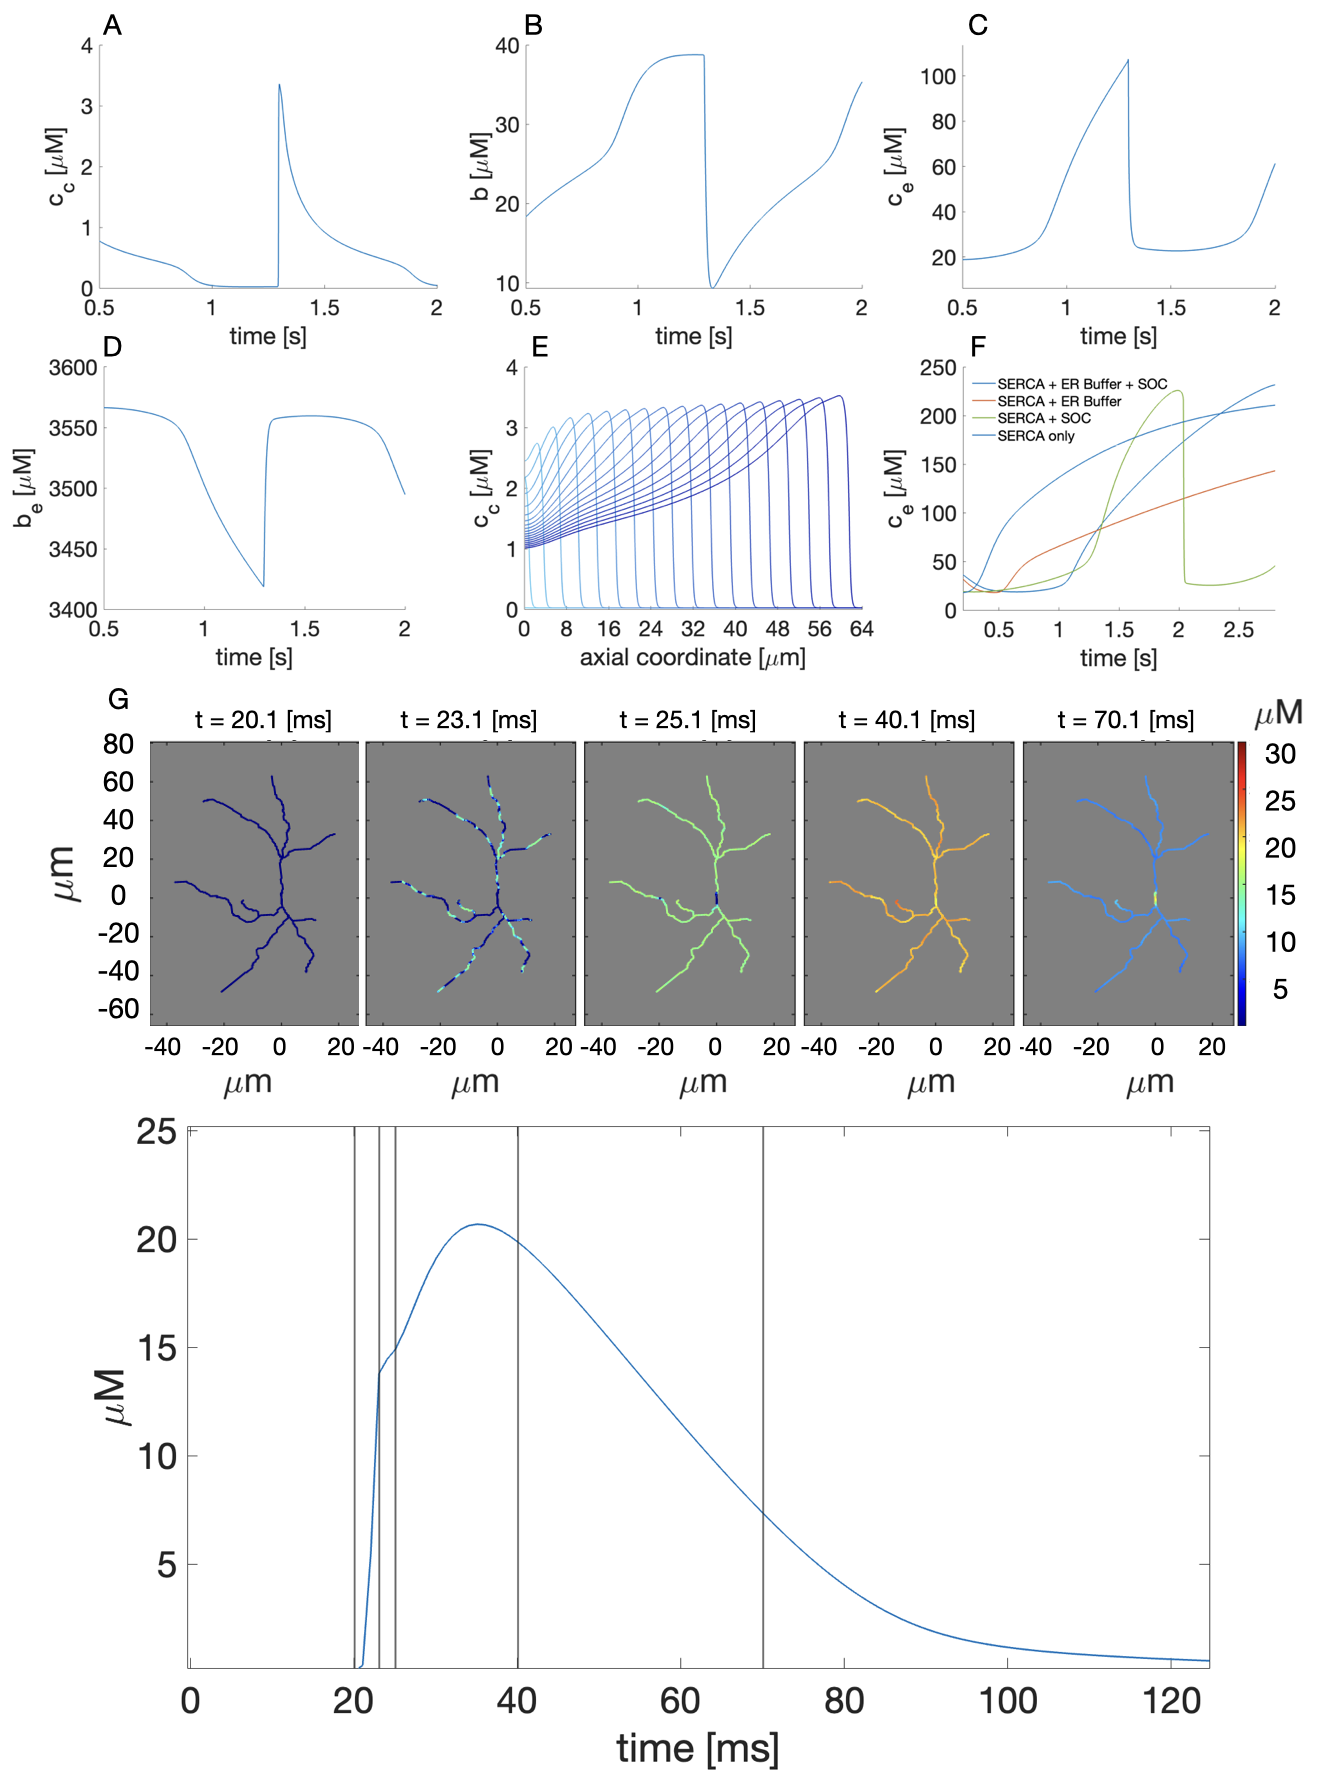
\includegraphics[width=0.9\textwidth]{Figures/basicPlotsFinal5.png}
    \caption{Dynamics is on unbranched neurite. (A-D) Concentration profiles for all modeled species measured at the soma. As the calcium wave reaches the soma, there is a spike in cytosolic \Ca concentration (A). This spike corresponds to a reduction in free CalB (B) as a result of fast buffering action of CalB on excess calcium in the cytoplasm rapidly forming CalB\Ca complex. The calcium-induced calcium response causes instant release of ER \Ca ($c_e$) into cytosol seen as massive dip in $c_e$ (C). The decrease in $c_e$ triggers release of \Ca bound to CalR ($b_e$) thereby increasing free CalR concentration in ER (D), (E) Stable calcium wave propagating through neurite cytoplasm translates and carries electrical signal from synapses to nucleus. The wave travels at the speed of approximately $0.5~\mu m/ms$. Each line represents $7.5$ ms time difference from each other,  (F) ER refilling is mediated SERCA channels along with Store operated channels. Additionally, huge amount of \Ca is stored as buffered \Ca by CalR which is released instantly as ER discharges \Ca into cytoplasm. Combined, these three mechanisms ensures that ER holds enough \Ca to release upon repeated activations. Neuronal response to stimulation of $1000$ synaptic junctions. (G) \textbf{Top:} The evolution of calcium wave over the neuron. The color represents cytosolic calcium concentration. Initially, $c_c$ is low at $50~nM$. The plot at $t=23.1~ms$ demonstrates triggering/stimulation of synapses at various locations of neuronal dendrites causing initiation of many calcium waves. These calcium waves travels throughout the body of neuron leading to increase in $c_c$ (at $t=25.1~ms$ and $t=40.1~ms$). Once the wave passes, the $c_c$ begins to fall to equilibrium state ($t=70.1~ms$).
    \textbf{Bottom:} Cytosolic calcium concentration at the soma over the simulation period. Each vertical line corresponds to the snapshot time in top panel.}
    \label{fig:BasicPlots}
\end{figure}


%****************************************%
\subsection{Modeling Electrical Dynamics} 
Electrical neuronal activity was modeled with the classical Hodgkin-Huxley equations \cite{Grein2014,Hodgkin1952A,Hodgkin1952B,Hodgkin1952C,Hodgkin1952D,Hodgkin1952E}, including explicit terms for sodium, potassium, and calcium ions:
\begin{align}\label{eqn:HH}
    C\frac{\partial V}{\partial t} = \frac{1}{R_{ax}}\frac{\partial V}{\partial x}\left( a(x) \frac{\partial V}{\partial x}\right)+I_{HH}(V,n,m,h)+I_{CaF}(V,c_c,x,y).
\end{align}
Here, $V$ is the membrane potential, $C$ the membrane capacitance, $a$ the neurite radius, $R_{ax}$ the axial resistance of the neurite, $I_{HH}(\cdot)$ the ionic current contribution from sodium, potassium, and leak, and $I_{CaF}(\cdot)$ is the fast $\textrm{Ca}^{2+}$ current contribution. The state variables for the potassium and sodium channels are given by $n$ for potassium, and $m,h$ for sodium. For the fast $\textrm{Ca}^{2+}$ current the variables $x,y$ denote the state variables.
The ionic current contribution $I_{HH}(\cdot)$ is given below for completion:
\begin{equation*}
    I_{HH}(V,n,m,h)=\bar{g}_Kn^4(V_K-V)+\bar{g}_{Na}m^3h(V_{Na}-V)+\bar{g}_l(V_l-V).
\end{equation*}
Here, $n$, $m$, and $h$ are the state variables for potassium ($n$) and sodium ($m,h$). The last term is the leakage term for ions not directly accounted for. The variables $\bar{g}_K$ and $\bar{g}_{Na}$ correspond to the maximum conductance for the potassium and sodium ion channels, respectively. The variable $\bar{g}_l$ is the leak conductance. The variables $V_K$, $V_{Na}$, and $V_l$ are the potassium, sodium, and leak reversal potentials, respectively. Equation \cref{eqn:HH} couples to the state ODEs, which we provide below:
\begin{align*}
    \frac{dn}{dt} &= \alpha_n(V)(1-n)-\beta_n(V)n,\\
    \frac{dm}{dt} &= \alpha_m(V)(1-m)-\beta_m(V)m,\\
    \frac{dh}{dt} &= \alpha_h(V)(1-h)-\beta_h(V)h,
\end{align*}
where the functions $\alpha_i(\cdot)$ and $\beta_i(\cdot)$, with $i\in \{n,m,h\}$, are rate functions. Below we provide the rate functions for completion, borrowed from \cite{Pospischil2008, rosado2022}:
\begin{align*}
    \alpha_n(V)&=\frac{-0.32(V-15)}{\textrm{exp}\left(\frac{15-V}{5}\right)-1},\ \ \ \ \beta_n(V)=0.5\ \textrm{exp}\left(\frac{10-V}{40}\right),\\[8pt]
    \alpha_m(V)&= \frac{-0.32(V-13)}{\textrm{exp}\left(\frac{13-V}{4}\right)-1},\ \ \ \ \beta_m(V)=\frac{0.28(V-40)}{\textrm{exp}\left(\frac{V-40}{5}\right)-1},\\[8pt]
    \alpha_h(V)&= 0.128\ \textrm{exp}\left(\frac{17-V}{18}\right), \ \ \ \ \beta_h(V)=\frac{4}{\textrm{exp}\left(\frac{40-V}{5}\right)+1}\cdot
\end{align*}
For the fast \Ca current contribution we borrow equations from \cite{proto1998,koch1989methods}, where
\begin{equation*}
I_{CaF}(V,c_c,\sigma,\rho)=\bar{g}_{Ca}\sigma\rho(V_{Ca}-V),    
\end{equation*}
and $V_{Ca}$ is the \Ca-dependent reversal potential, given by the Nernst equation
\begin{equation*}
    V_{Ca}=12.5\cdot\log\left(\frac{c_o}{c_c}\right).
\end{equation*}
The variables $\sigma$ and $\rho$ have corresponding equations, where
\begin{equation*}
    \frac{d\sigma}{dt}=\frac{\sigma_\infty-\sigma}{\tau_\sigma}
\end{equation*}
is the governing ODE with
\begin{align*}
    \tau_\sigma=\frac{7.8}{\textrm{exp}((V+6)/16)+\textrm{exp}(-(
    V+6)/16)},\ \ \ \ \sigma_\infty=\frac{1}{1+\textrm{exp}(-(V-3)/8)}.
\end{align*}
The variable $\rho$ is computed by
\begin{equation*}
    \rho(c_c)=\frac{K}{K+c_c},
\end{equation*}
with $K$ fixed (see Table SM2). Note, the term $I_{CaF}(\cdot)$ couples the calcium model to the electrical model.


%*********************************%
\subsection{Modeling synapses} \label{sec:modeling-synapses} 
In Sec.~\ref{sec:experiments} we make use of a test geometry, which is an unbranched neurite, and an anatomical neuron reconstruction. For the unbranched neurite, we place one synapse at the first point (left most point) of the geometry such that there is only one synaptic \Ca source. 

For the full neuron geometry, let $S$ be the total number of synapses that are distributed across the neuron. This will include healthy and leaky synapses, $S=H+L$, where $H$ is the number of healthy and active synapses and $L$ is the number of leaky synapses. The neuronal geometry is represented as a discrete set of nodes with a connectivity graph and neurite diameters attached to each node, where the neuron's graph $G$ contains $N$ nodes. We distribute the number of synapses $S$ across the $N$ nodes. For example, at node $x_i$ there are $H_i,L_i$ healthy and leaky synapses, respectively. It is possible for some nodes not to contain synapses ($H_i=L_i=0$) which may occur if $N \gg S$. Therefore, $S=\sum_{i=1}^NH_i+L_i$ and synaptic influx is modelled by eq.~\cref{eqn:syn1}. 

In order to model pure synapse loss we do not include leaky terms associated with amyloid $\beta$ and only modify the value of $H_i$~(see Sec.~\ref{sec:experiments}. Synaptic influx at only healthy synapses ($H$) are modeled as leaky synpases ($L$) are modeled by deactivating leaky synapses. 
For an unbranched neurite the same applies with $H_1=1$ and there is no synapse loss.

The leakage flux associated with amyloid $\beta$ is added to $J_{l,p}(c_c)$ if a synapse is set as leaky. This mimics the constant leak into the cytoplasm at equilibrium by amyloid $\beta$ clustering (see Sec.~\ref{sec:leaky-synapses}). The flux $J_{l,p}(c_c)$ then becomes
\begin{align*}
    J_{l,p}(c_c)&=v_{l,p}\cdot(c_o-c_c) + \delta \cdot J_{A \beta},
\end{align*}
where $\delta ~=~ 1$ if the node contains leaky synapses and $\delta ~=~ 0$ otherwise. In the unbranched neurite test geometry, while simulating leakiness, every third node is set as leaky.
In order to model synapse loss with leakage in full neuron geometry, $\delta$ for synapses in $L$ is set to $1$.
At the leakage site, $J_{A\beta}$ is continuously added throughout the simulation to mimic leakage occurring in biologically realistic scenarios. 

%**********************************%
\subsection{Neuron reconstructions} \label{sec:neuron-reconstructions}
Simulations were carried out on two geometries, (1) an unbranched, symmetric cable (see Fig.~\ref{fig:Illustration}A), representing a dendrite with a length of 64 $\mu m$, a dendrite diameter of $0.8 ~\mu m$ and ER diameter of $0.3~\mu m$ and (2) an anatomical reconstruction of an adult female mouse brain-stem neuron \cite{Bertels2021} borrowed from \href{http://neuromorpho.org}{NeuroMorpho.org} \cite{Ascoli2007}, with identification $\texttt{NMO\_150605}$. While the simplified dendritic geometry was used for illustrating the fundamental dynamics that emerge from the coupled electro-calcium model in Sec.~\ref{sec:calcium-dynamics-membrane-transport}--\ref{sec:modeling-synapses}, the neuronal geometry was used to study the effects of changes in parameters affected by AD in a realistic setting.

Both geometries were processed to have a quasi-uniform edge length defined by $\Delta x$ and therefore the number of nodes is given by $N = \lfloor\frac{l}{\Delta x}\rfloor + 1$, $l$ being the total dendritic length. We then chose the edge length to be $\Delta x_m = 2^{-m+2} ~\mu m$ with $m=0,1,2,\ldots$. These mesh hierarchies were used to carry out a numerical convergence analysis (see Sec.~\ref{sec:numerical-methods}).
\iffalse
We began our analysis by generating artificial 1D beam geometries to determine the numerical accuracy of the implementations. These geometries model a 1D neurite plasma membrane of length 64 $\mu m$ with a prescribed uniform $\Delta x$ for the edge length. For a given $\Delta x$, the number of nodes $N$ is given by $N=\lfloor\frac{64}{\Delta x}\rfloor$ We generated refinements of this geometry where a refinement-$m$ yields a 1D beam with edge length $\Delta x_m = 2^{-m+1}$. We made refinements- $0,1,2,3,4$; therefore, we obtain geometries with $\Delta x\in [2.0, 1.0, 0.5,0.25,0.125]\ \mu m$. These 1D refinements were used to determine the level of spatial resolution, i.e. $\Delta x$, for \textit{sufficient} accuracy. Additionally, we executed simulations with uniform radius of the neurite, that is to say for each node on the 1D beam with $N$ nodes the radius $r_i$ at $x_i$ is equal to $r$ i.e. $r_1 =r_2=\cdots=r_N=r$. The non-uniform radii case will be discussed in Section \ref{sec:experiments}. 
\fi
All geometries used in this study were saved in \texttt{.swc} format, which is one of the standard readable text file formats for saving the graph connectivity and spatial structures of neuroanatomical reconstructions \cite{Stockley1993}. In this format neuron morphologies are saved as a table which contains $N$ rows corresponding to each node of the geometry, and each row contains the following information
\begin{center}
    \texttt{ID\quad TYPE\quad X\quad Y\quad Z\quad RADIUS\quad PID}
\end{center}
where \texttt{ID} is the node id number ranging from $[1,N]$. \texttt{TYPE} identifies the neuronal compartment, where e.g.~the value 1 denotes the soma and 2 a dendrite (note, other identifiers exist). \texttt{X,Y,Z} are the spatial coordinates of the node, \texttt{RADIUS} is the radius of the neurite at the node, and \texttt{PID} is the parent id of the node. Note, that the set of $N-1$ pairs $(\texttt{PID},\texttt{ID})$ define the set of edges of the neuron graph, which defines the connectivity map of the geometry.
  

%*****************************%
\subsection{Numerical Methods} \label{sec:numerical-methods}
To solve the model equations presented in Sec.~\ref{sec:calcium-dynamics-membrane-transport}--\ref{sec:modeling-synapses} on discrete geometries (see Sec.~\ref{sec:neuron-reconstructions}) we employed a semi-implicit time stepping scheme with finite difference discretization of the spatial domain. Equations \cref{eqn:diffcc}--\cref{eqn:diffbe}, and \cref{eqn:HH} can each be expressed as 
\begin{align*}
X_t &= AX + BX\\
s_t &= 0s + Fs.
\end{align*}
where $A$ is the discretization of the second order differential operator $\partial_{xx}$ and $B$ is the reaction function. For the \Ca equations $B$ contains the current influx terms and any additional reaction terms, and for the Hodgkin-Huxley model equation \cref{eqn:HH} the $B$ term would be the sum of the ion currents. Note, in the first equation $X=(c_c,c_e,b,b_e)$ while the second equation stands for the state variables used in the Hodgkin-Huxley model, i.e. $s=(n,m,h)$. The implicit-explicit time stepping method we implemented is the semi-implicit backward differetiation formula of second order (SBDF2) \cite{Seibold2019-df,Albi2021,rosado2022},  which is given by the update rule
\[
\frac{3}{2}X^{i+1}-2X^i+\frac{1}{2}X^{i-1} = \Delta t A X^{i+1}+2\Delta t BX^i-\Delta t B X^{i-1},
\]
which yields
\[
\left(I-\frac{2}{3}\Delta t A \right) X^{i+1} = \frac{4}{3}X^i+\frac{4}{3}\Delta t BX^i-\frac{1}{3}X^{i-1}-\frac{2}{3}\Delta t BX^{i-1}.
\]
For the state variables a matrix of zeros is used for the right hand side and is written as
\[
s^{i+1} = \frac{4}{3}s^i+\frac{4}{3}\Delta t Fs^i-\frac{1}{3}s^{i-1}-\frac{2}{3}\Delta t Fs^{i-1}.
\]
For both equations, one needs to know the current state $X^i,s^i$ and the prior state $X^{i-1},s^{i-1}$ to compute the next states.

For the spatial discretization, we consider the 1D nature of the geometry and apply finite differences \cite{LeVeque2007} at every node of the geometry. As an example we consider a non-branched piece of dendrite with nodes $x_{-1}, x_0,$ and $x_1$. Then the approximation to the second order differential operator at location $x_0$, with diffusion coefficient $D$, is given by
\begin{equation*}
    D\frac{\partial^2 u_0}{\partial x^2}\approx \frac{D}{(\Delta x)^2}\left(u_{-1}-2u_{0}+u_1\right)
\end{equation*}
where $u$ corresponds to the ion concentration variables, i.e. $c_c, c_e$\ldots etc. However, a neuron contains branching locations; therefore, we use a generalized form of the above approximation for a branch point $x_i$ with neighbors indexed by $j\in\mathcal{N}$, where $\mathcal{N}$ contains the indices of the nodes that are neighbors to node $i$. Additionally, we allow non-uniform edge lengths. The approximation to the second derivative at a branch point $x_i$ is given by (see \cite{calsim}):
\begin{equation*}
    D\frac{\partial^2 u_i}{\partial x^2}\approx \frac{2D}{\displaystyle\sum_{j\in \mathcal{N}}(\Delta x)_j}\left(\sum_{j\in\mathcal{N}}\frac{u_j}{(\Delta x)_j}-u_i\sum_{j\in\mathcal{N}}\frac{1}{(\Delta x)_j}\right),
\end{equation*}
where $(\Delta x)_j=\lVert x_i-x_j\rVert_2$, the Euclidean distance between the two nodes $x_i$ and $x_j$. The derivation and example cases of the above approximation to the second order derivative can be also be found in \cite{calsim,rosado2022}. Convergence analysis was conducted with varying levels of refinements $m=1-5$. The refinement level is associated with time steps $\Delta t_m = 160,80,40,20,10~ms$) and edge length $\Delta x_m = 2,1,0.5,0.25,0.125 ~\mu m$.  The result of convergence analysis is available in Fig. SM1. Refinement level $1$ and $2$ were too coarse for convergence (not plotted). Refinement $3-5$ show convergence and the selected refinement level was $5$ ($\Delta x = 0.125~\mu m$ and $\Delta t=10~ms$) for all simulations presented in Sec.~\ref{sec:experiments}.



%**************************************************************************%
%NEW SECTION$
%**************************************************************************%

\section{Biological Results}
\label{sec:experiments}
Using the model described in Sec.~\ref{sec:model} we studied the effect of parameters that are known to change during AD. We designed a baseline ``healthy'' neuron by randomly distributing 1,000 synapses on the dendritic tree of a neuron selected from NeuroMorpho.org \cite{Ascoli2007, Bertels2021}. Synapses were then activated randomly within a defined time window of 10 ms. We used a stimulation frequency of 1Hz and 5Hz to cover the frequency range known to be relevant for learning and plasticity \cite{dolmetsch1997differential,dolmetsch1998calcium,kupzig2005frequencies} and studied the effect of different frequencies on somatic calcium responses (see Sec.~\ref{sec:frequency-filtering}). The baseline neuron simulations used the default parameters listed in Table SM1. To illustrate the fundamental calcium dynamics of the model in Sec.~\ref{sec:model} and the influence of specific parameter variations on synapse to soma communication we also used a simple test geometry, an unbranched neurite with constant dendritic and ER radius.

In this study we focused on three major parameters: (1) synapse loss \cite{subramanian2020synaptic,terry1991physical,dekosky1996structural}, (2) calcium leaks at deteriorated synapses \cite{demuro2010calcium,demuro2011single,itkin2011calcium, lin1999amyloid, kawahara1997alzheimer, quist2005amyloid,di2014interaction,di2016common,lal2007amyloid}, and (3) downregulation of the calcium buffer calbindin in the cytosol \cite{iacopino1990specific, kook2014crucial, crapper1987calmodulin,palop2003neuronal}. Synapse loss is a well documented effect seen in neurodegeneration  \cite{subramanian2020synaptic,terry1991physical,dekosky1996structural}. This was modeled by pure removal of synapses from the pool of active synapses (see Sec.~\ref{sec:synapse-loss}) and then by additionally adding a \Ca leakage term at deteriorated, leaky, synapses (see Sec.~\ref{sec:leaky-synapses}). Lastly, we studied what effect a $25$\% downregulation of Calbindin has on \Ca signaling in diseased neurons (see Sec.~\ref{sec:calbindin-downregulation}). 



\subsection{Neuronal frequency filtering from synapse to soma}\label{sec:frequency-filtering}
\begin{figure}[!htb]
    \centering
    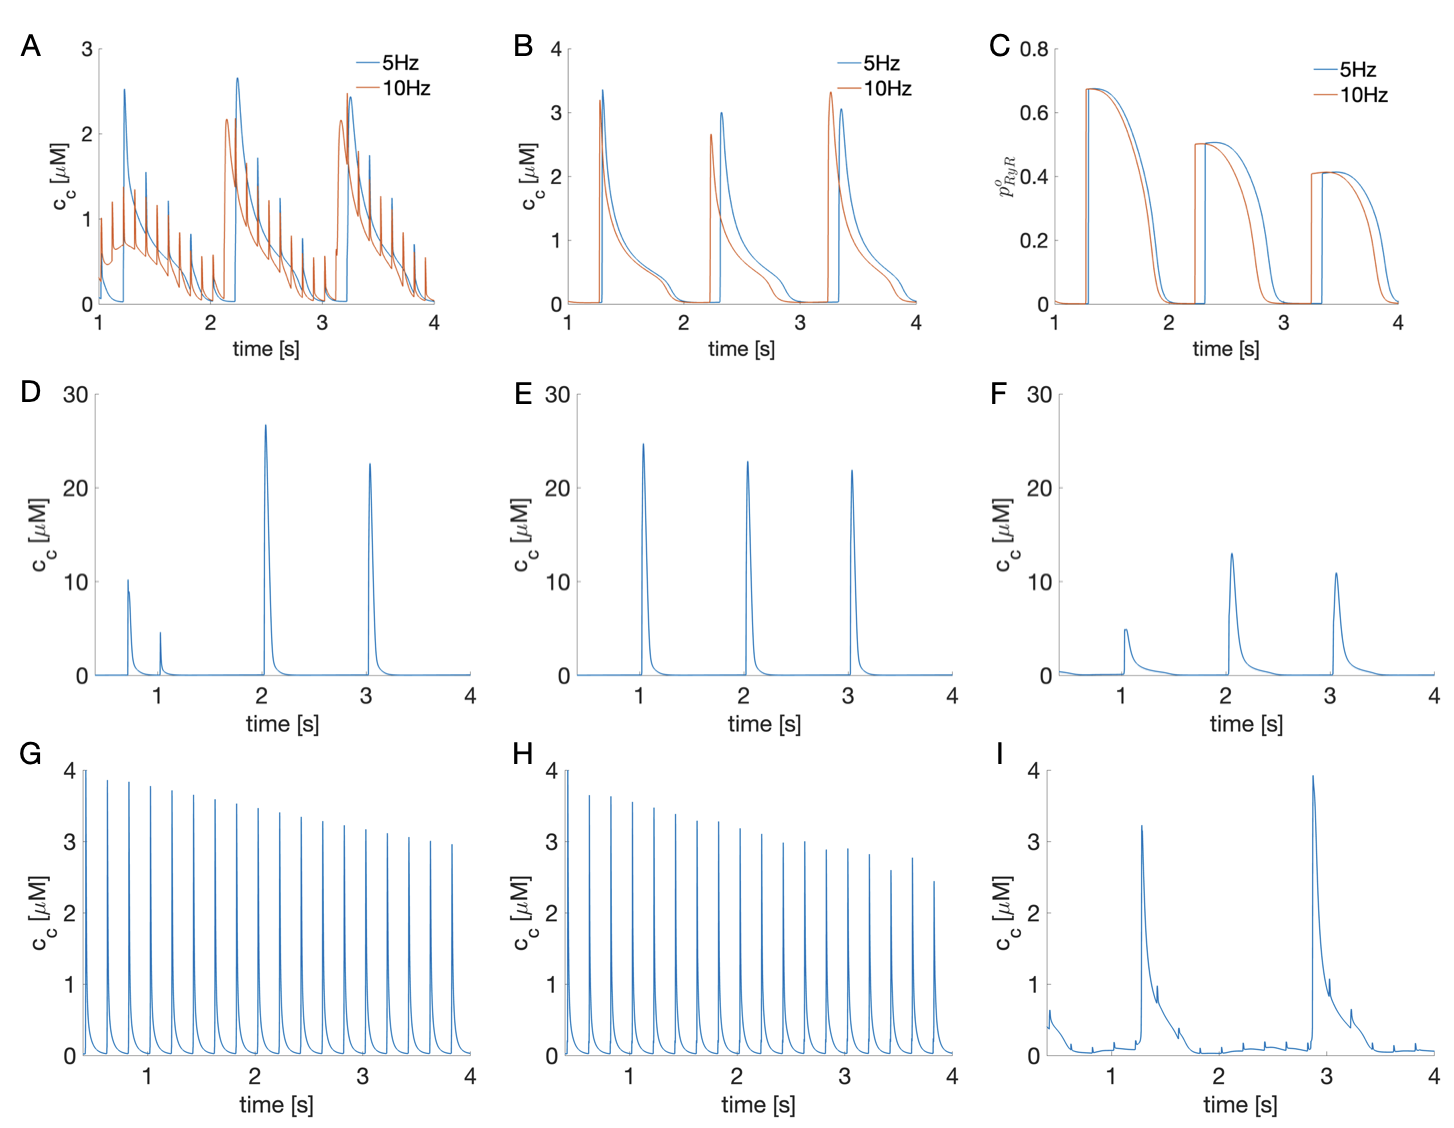
\includegraphics[width=12cm]{Figures/frequency-filter-final1.png}
    \caption{$Ca^{2+}$ response to varying levels of stimulation frequency at soma. (A-C) Response to $5$ and $10$ Hz stimulation on an unbranched neurite. (A) represents the $Ca^{2+}$ profile of the stimulated synapse at $5$ and $10$ Hz. The input frequencies are filtered down to $1$ Hz response at soma (B). This occurs due to the kinetics of RyR channels open state probability which takes almost $1$ second to reduce down to zero after each wave event (C). (D-I) Response to varying levels of stimulation frequency in a full neuron at two branch points (points $2$ and $8$ in Fig. \ref{fig:Illustration}B.) and soma. (D-F) $1$ Hz stimulus response at two branching points (D and E) and at the soma (F). While the $1$ Hz stimulus frequency is detectable at all locations, most importantly at the soma, one can observe the dendritic tree resolving the high-frequency stimulus. (G-I) $5$ Hz stimulus frequency travelling through the tree gets filtered to $3$ Hz at the branch points (G and H) which further propagating towards and reaching the soma responds at a roughly $1$ Hz frequency (I).}
    \label{fig:frequency-filter}
\end{figure}
Before modifying any biophysical parameters, we were interested in analysing the effect of different synapse stimulation frequencies on calcium signaling along the dendrites to the soma. Using the simple test geometry we stimulated at one end of the unbranched neurite and measured at the mid point (considered the soma). In Fig.~\ref{fig:frequency-filter}A we see that at the location of stimulation calcium signals recover the $1$ Hz stimulus, as well as the $5$ Hz stimulus, although calcium amplitudes at the higher frequency are reduced. Moving away from the activation site, the ``simple'' neuron can reliably recover the $1$ Hz frequency, but filters the 
$5$ Hz stimulus and produces a roughly $1$ Hz response. 

The reason for this frequency filtering effect appears to lie in the kinetics of the ryanodine receptors. For a stable wave response to occur, a strong RyR current is needed, which occurs when $p^{o}_{RyR}$ increases rapidly. One $p^{o}_{RyR}$ cycle takes approximately $1$ second. 
During this time period, any synaptic event has reduced impact on $p^{o}_{RyR}$, which leads to an abortive wave.

This is illustrated in Fig.~\ref{fig:frequency-filter}A-C. 
Fig.~\ref{fig:frequency-filter}A demonstrates \cc response to a $5$ and $10$ Hz input frequency at the synapse of the unbranched neurite. The responses to these inputs are filtered to $1$ Hz at the soma, i.e., at the center node of the neurite (Fig.~\ref{fig:frequency-filter}B). 
Fig.~\ref{fig:frequency-filter}C shows $p_{RyR}^o$ at the soma. In both cases $p_{RyR}^o$ cycle time is $\approx$ 1s. This makes the site unresponsive to incoming signals until $p^{o}_{RyR}$ reaches equilibrium, after which the neurite can respond again.

We were interested whether this frequency filtering effect carries over to an actual neuron and repeated the computational experiment using a reconstructed neuron, see Fig.~\ref{fig:frequency-filter}D-I, on which we placed $1,000$ synapses randomly and triggered these at a $1$ and $5$ Hz frequency. We measured \cc response at branch points 2 and 8 and at the soma (see Fig.~\ref{fig:Illustration}B,C). As seen in Fig.~\ref{fig:frequency-filter}D, the neuron, independent of measurement site, is able to respond with a $1$ Hz calcium signal that propagates towards the soma. However, when the stimulation frequency is increased to $5$ Hz, we see that dendritic branches respond at roughly $3$ Hz, which decays to $1$ Hz responses at the soma (see Fig.~\ref{fig:frequency-filter}G-I).  


\subsection{Effect of synapse loss on intracellular \Ca dynamics}\label{sec:synapse-loss}


\begin{figure}[!htb]
    \centering
    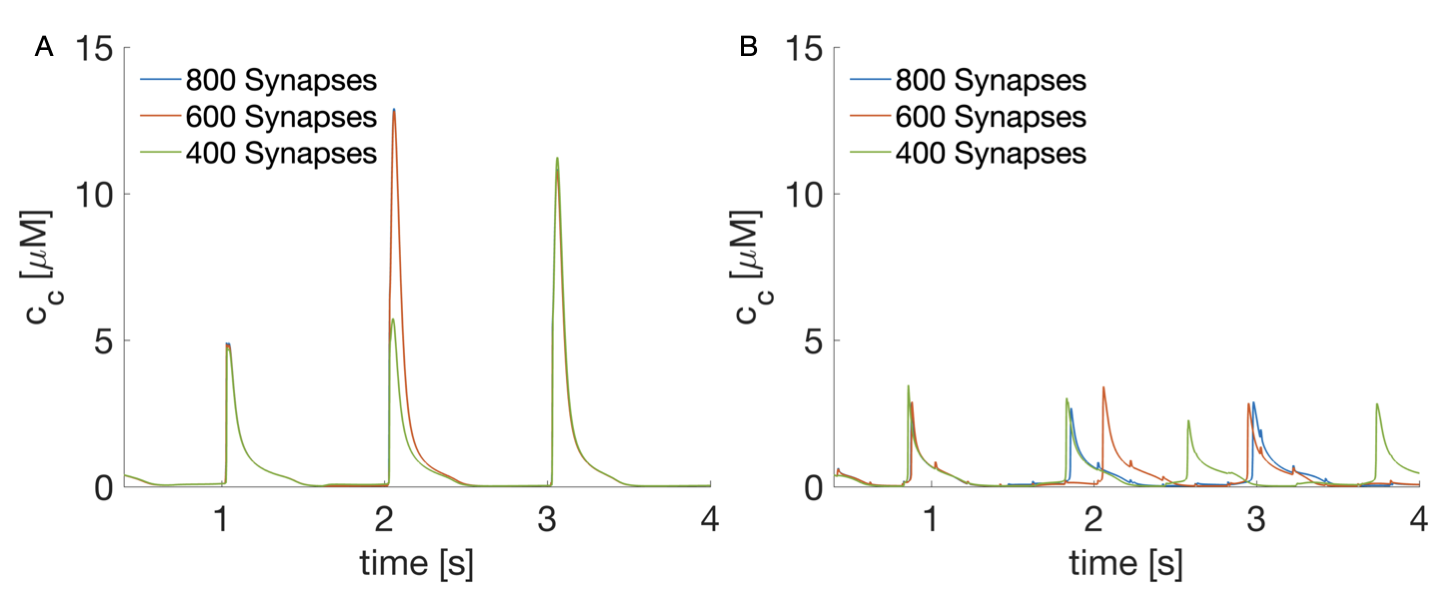
\includegraphics[width=12cm]{Figures/synapse-loss-final1.png}
    \caption{\Ca response observed at soma at various levels of synapses loss. Originally, $800$ active synapses (low level pathology) are considered from which $200$ synapses were removed serially leaving $600$ (medium level pathology) and $400$ (high level pathology) active synapses . $1$ Hz stimulus response (A) and $5$ Hz stimulus response (B) were not significantly affected as a result of synapse loss.}
    \label{fig:synapse-loss}
\end{figure}

Synapse loss is a well-documented part of AD and other neurodegenerative processes. Chemical synapses operate at multiple functional scales, e.g. transmitting electrical signals through release of neurotransmitters, but also by controlling \Ca entry into the cytosol at active post-synaptic sites. An influx of \Ca at the postsynaptic density can induce long-range \Ca signals, e.g. \Ca waves, by calcium-induced calcium-release (CICR) cascades at the endoplasmic membrane \cite{verkhratsky1996calcium,berridge2003calcium}. Post-synaptic spine to dendrite communication, controlled by the intracellular organization and the stability of dendritic \Ca waves has been studied in the past \cite{Breit2018,Queisser2018}. 

In healthy neurons, with an active and functioning synapse population, synapse to soma \Ca communication should be possible, as seen in Fig.~\ref{fig:frequency-filter}. However, under conditions where the pool of active synapses is reduced, as in AD, a communication disruption between active synapses and the soma could potentially occur. This would have major implications for cell survival, since \Ca signals at the soma trigger biochemical cascades in the cell nucleus relevant for cell survival \cite{berridge2003calcium,lohmann2005regulation,michaelsen2010calcium,redmond2005regulation}. There, amplitude, duration, and frequency of the \Ca signal regulates gene transcription responses \textcolor{black}{\cite{dolmetsch1998calcium,li1998cell,zhou2015calcium}}. 

We were therefore interested in studying the somatic \Ca response when iteratively removing synapses from the active pool. In Fig.~\ref{fig:synapse-loss} we show the somatic \Ca response for a low level pathology state ($800$ active synapses), medium level pathology state ($600$ active synapses), and high level pathology state ($400$ active synapses) at a 1Hz and 5Hz stimulation frequency. While there are observable fluctuations in the peak amplitudes of the signals and in the 5Hz case shifts in the frequency (and both could influence downstream biochemical cascades), \Ca signals are able to reach the soma even under significantly reduced active synapse scenarios. From the computational experiments it appears that neurons, with their intricate intracellular \Ca machinery, is well equipped to compensate significant synapse loss during neurodegeneration. 

\iffalse
\textcolor{red}{To keep consistency with other figure captions should this caption be the number of active synapses? 600 and 400 (200 leaky synapses would indicate 800 active synapses but there was an anomoly for the 5hz so we changed it to be 600 active synapses)}
\fi
\subsection{Leaky synapses disrupt synapse to nucleus pathway}\label{sec:leaky-synapses}
\begin{figure}[!htb]
    \centering
    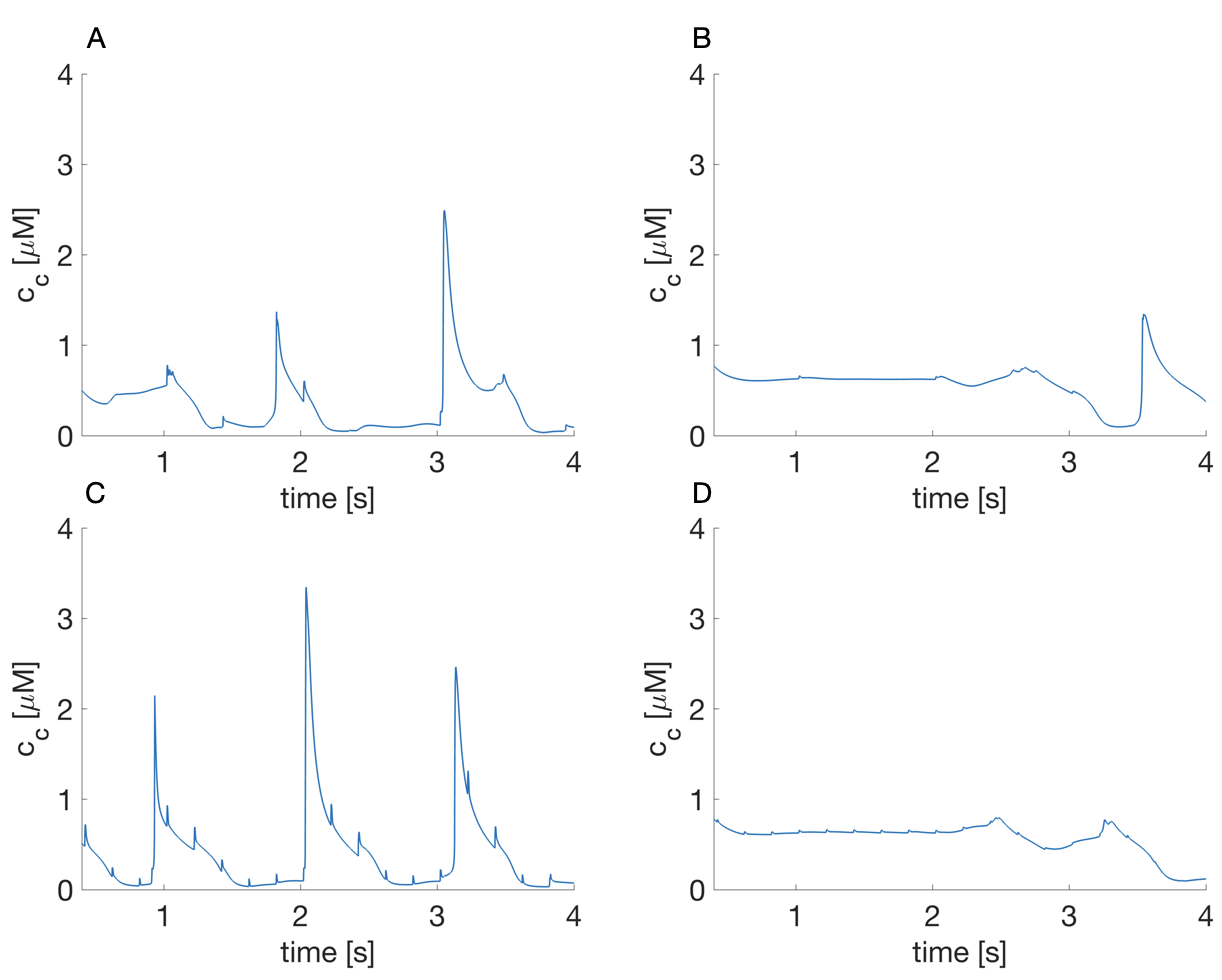
\includegraphics[width=12cm]{Figures/leaky-synapses-final1.png}
    \caption{
    Somatic \Ca response to synapse loss coupled with leakage caused due to amyloid $\beta$ pores. The $1$ Hz and $5$ Hz stimulus response with $600$ active synapses (medium level pathology, A and C respectively) disrupts signalling minimally. However, the $1$ Hz and $5$ Hz stimulus response with $400$ active synapses (high level pathology, B and D respectively) causes  significant disruptions to signalling. This is caused by accumulation of \Ca in cytoplasm thereby increasing equilibrium cytoplasmic \Ca levels.} 
    \label{fig:leaky-synapses}
\end{figure}
Calcium entry into the cytoplasm from the extracellular space is controlled by calcium exchangers embedded in the plasma membrane \cite{brini2011plasma,Graupner2003,Graupner2005}. In AD, it has been shown that the plasma membrane at deteriorated synaptic contacts can become leaky to \Ca \cite{demuro2010calcium,demuro2011single,itkin2011calcium, lin1999amyloid, kawahara1997alzheimer, quist2005amyloid,di2014interaction,di2016common,lal2007amyloid} leading to \Ca accumulation in the cytoplasm. This disrupts the CICR release mechanism responsible for intracellular \Ca communication. 

In addition to modeling synapse loss as described in Sec.~\ref{sec:synapse-loss}, we made lost synapses leaky to \Ca by introducing a \Ca leakage term (see Sec.~\ref{sec:model}). We again incrementally decreased the pool of active synapses and made removed synapses leaky for \Ca. Fig.~\ref{fig:leaky-synapses} shows the results for $800$ active synapses ($200$ leaky synapses, low level pathology) to $400$ active ($600$ leaky, high level pathology) at a $1$ Hz and $5$Hz stimulation frequency. With the decrease in active synapses, we initially observe similar results as described in Sec.~\ref{sec:synapse-loss}. Peak \Ca amplitudes decrease with decrease of active synapses and in the $5$ Hz case a change in response frequency. However, when reaching roughly $400$ active synapse sites (or $600$ leaky, high level pathology), the somatic \Ca signal is entirely disrupted, i.e. no oscillating \Ca signal with distinct peak amplitudes are measurable. We describe this phenomenon as synapse to soma communication breakdown. 

The accumulation of \Ca in the cytoplasm causes $p^o_{RyR}$ to reach equilibrium state (i.e. zero) slowly. This maintains $p^o_{RyR}$ at an elevated level and makes the ER unresponsive to a new activation flux. This significantly reduces strength of $j_{RyR}$ which is the primary contributor to the spike in cytoplasmic \Ca needed for driving a \Ca wave/signal. Fig. SM2 demonstrates this phenomenon of accumulated cytosolic \Ca in an unbranched neurite with leaky synapses leading to elevated $p^o_{RyR}$ levels over time in comparison to a neurite with non-leaky synapse states. 

While neurons can apparently tolerate a significant degree of synapse loss without compromising synapse to soma communication, the introduction of \Ca leakiness at deteriorated synapses disrupts the intracellular \Ca signaling to the extent that somatic \Ca responses to low and high-frequency inputs are no longer measurable. 

\subsection{Downregulation of \Ca buffer Calbindin partially mitigates signal disruption from synapse loss}
\label{sec:calbindin-downregulation}
The last parameter we were interested in for this study was the intracellular Calbindin \Ca buffer concentration. The concentration in healthy and AD neurons has been experimentally studied \cite{iacopino1990specific, kook2014crucial, crapper1987calmodulin,palop2003neuronal} and a reduction in Calbindin concentration is documented in diseased neurons. We therefore reduced the basal Calbindin concentration by $25\%$ (pathological concentration) and repeated the simulations of synapse loss with synaptic calcium leaks. 

 In Fig.~\ref{fig:calbindin-reduction} we show the results for healthy and pathological Calbindin concentrations at 5Hz stimulation frequency. First, we identified the synapse number at which, under normal Calbindin concentrations, we see the onset of synapse to soma communication breakdown (which occurs at around $460$ active synapses). We then increased the number of active synapses to $470$ and noticed that while under normal Calbindin concentrations there is only a small recovery towards a healthy somatic response, a pathological (decreased) Calbindin concentration allows the neuron to produce more robust \Ca signals at the soma. 

Reduction in Calbindin has been observed in AD \cite{kook2014crucial}. Cytoplasmic Calbindin plays an important role not only in \Ca buffering, but also in inhibiting apoptotic pathways. Reduction in Calbindin concentration has been shown to exacerbate AD pathologies and increased propensity of a neuron to enter apoptosis \cite{kook2014crucial}. 
From this perspective the result that \Ca signalling is partially recovered by Calbindin reduction is exciting. 

As dysregulation of \Ca signaling is an important feature of AD pathology, targeting this disruption pathway could be the basis for an effective treatment modality for AD \cite{parys2018calcium}. It may be plausible that reduction of cytoplasmic Calbindin concentration could help neurons mitigate damage caused by elevated \Ca concentration in the cytoplasm. 

Whether this improved cell signaling is helpful or detrimental to neurons needs further investigation.
% Since a reduction of calcium buffering molecules would increase the concentration of free calcium in the cytosol and therefore exacerbate the effect of calcium leaking into the intracellular space, we expected this to worsen the synapse to soma communication breakdown. Yet, the contrary can be observed. \textcolor{red}{WHY?}.

\begin{figure}[!htb]
    \centering
    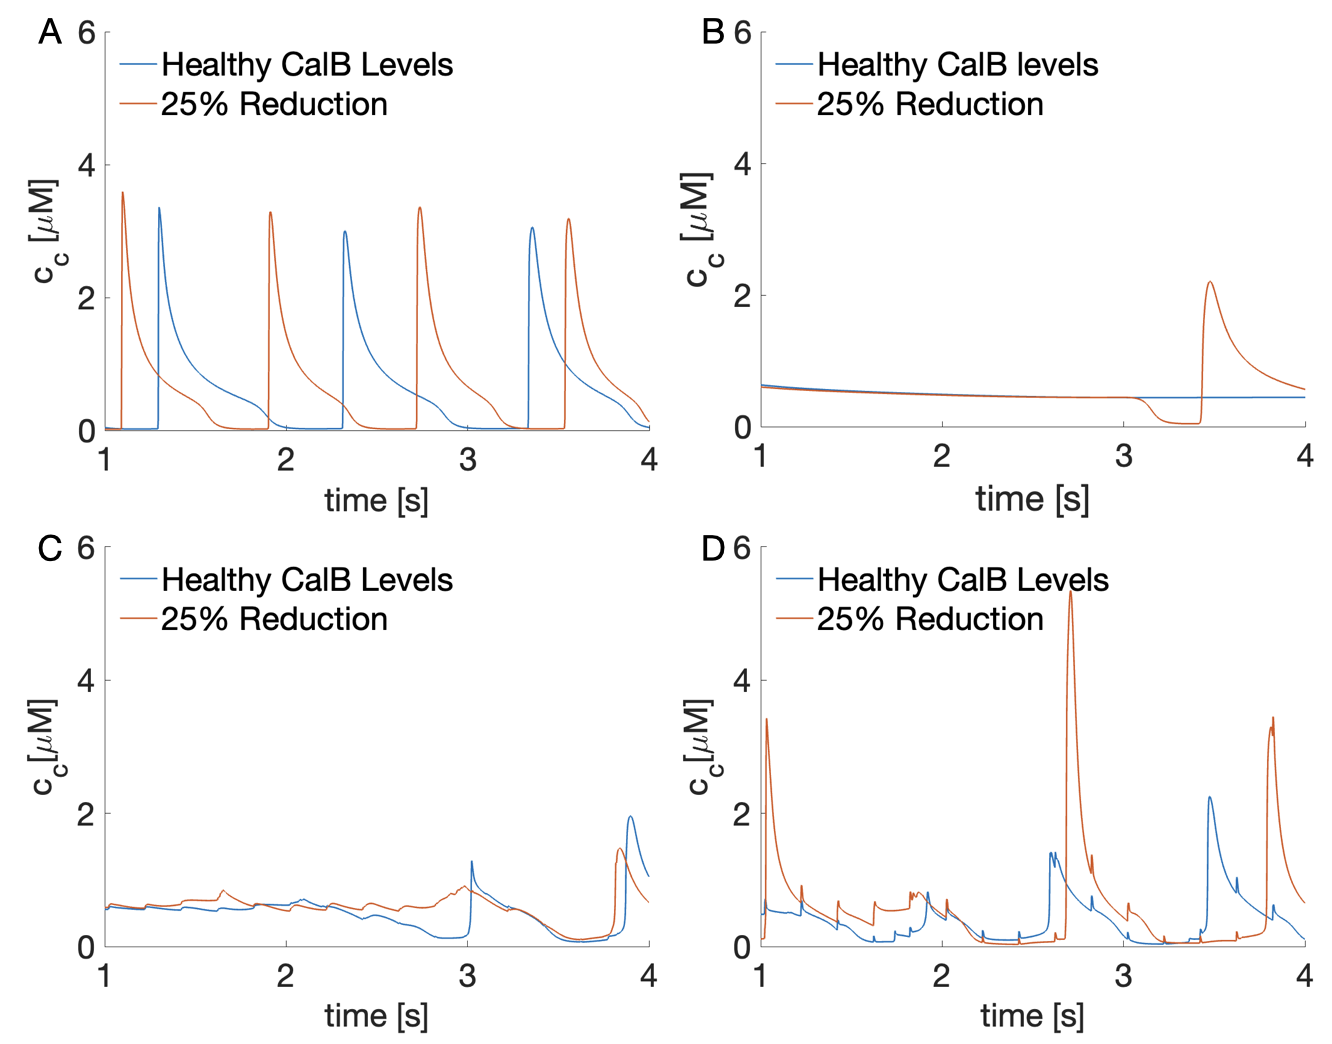
\includegraphics[width=12cm]{Figures/beam-and-calbreduction2.png}
    \caption{Somatic $Ca^{2+}$ response to downregulation of calbindin and synapse loss in an unbranched neurite (A-B) and full neuron geometry (C-D) at $5$ Hz stimulation. (A) Baseline experiment with no leakage indicates increased frequency response to stimulus at $25\%$ CalB reduction. (B) With leakage added, the wave responses at soma are delayed (compared to baseline) and only visible in pathological state in given simulation time. (C) The signalling is significantly disrupted in both healthy and pathological CalB concentration in full neuron geometry with $460$ active synapses ($540$ leaky synapses). (D) Signalling in partially recovered at $470$ active synapses ($530$ leaky synapses) when CalB is downregulated.} 
    \label{fig:calbindin-reduction}%-beam}
\end{figure}


%**************************************************************************%
%NEW SECTION$
%**************************************************************************%

\section{Discussion} \label{sec:discussion} 
In this paper, we present a biophysical model of coupled calcium and electrical dynamics in neurons. 
The \Ca model is based on a previously developed three-dimensional model for ultrastructural simulations in neuronal subcompartments \cite{Queisser2018,Breit2018,Rosadoplos2022}.
In order to extend simulations to full cells for synapse to soma signaling, without making computations prohibitively costly, we assumed rotational symmetry of dendritic and endoplasmic segments at segment length scale of $10^{-1}$ $\mu m$. 
The assumption of rotational symmetry allows us to derive a dimension-reduced version of the previous 3D model. 

Since the biological focus of the presented work was to study \Ca signaling to the soma under healthy and neuropathological conditions, the model was developed to include relevant \Ca exchange mechanisms embedded in the plasma- and endoplasmic membranes. Voltage-dependent \Ca channels bidirectionally couple the \Ca and electrical model, which is based on the standard Hodgkin-Huxley formalism. To correctly capture endoplasmic \Ca exchange with the cytosol under repeated synaptic stimulation, we incorporated known ER refilling mechanisms that operate on different time scales: slow SERCA pump refilling, medium store operated \Ca channel refilling, and fast reaction of endoplasmic bound \Ca to free \Ca ions. 

A reconstructed neuron from the NeuroMorpho.org \cite{Ascoli2007,Bertels2021} database was used to carry out simulations of cellular \Ca dynamics. The resulting system of PDEs and ODEs were solved by spatial discretization of the computational domain and the PDEs using a finite difference approach. To address computational cost we chose SBDF2 as our time stepping scheme to treat stiff and non-stiff components separately and to avoid additional stage-computations per time step. 

Using the developed biophysical model and computational framework we addressed the key question of how synapse to soma \Ca signals change due to pathology driven modulation of active synapse numbers, leakiness at deteriorated synapses and downregulation of \Ca buffering molecule Calbindin, all three modulations have been experimentally documented. This study revealed that pure synapse loss can be compensated well by neurons, although some changes in \Ca signal amplitudes, timing, and frequency can be observed. If deteriorated synapses become leaky to Ca$^{2+}$, which was modeled by an additional \Ca leakage term in the plasma membrane, and synapse loss becomes severe, synapse to soma communication breaks down, resulting in no controlled signals at the soma. This communication breakdown appears to be compensated to a certain extent by downregulation of Calbindin in the cytoplasm. 

In forthcoming research we plan to integrate a numerical optimization strategy and use healthy neuron synapse to soma \Ca dynamics to formulate an objective function. Optimizing biophysical parameters in the biophysical model, such as channel densities, ER size, and reaction rates towards healthy \Ca dynamics from a pathological state could lead to new insight into how medical intervention may designed to counter synapse deterioration. Additionally, while reduction in Calbindin may help in recovering \Ca signaling, it has also been reported that it aggravates AD pathologies \cite{kook2014crucial} due to its participation in many pathways including blocking apoptotic pathway. This requires further investigation and factored in to create a more realistic model.

%\section{Conclusions}
%\label{sec:conclusions}
%Some conclusions here.

%\appendix
%\section{An example appendix} 
%\lipsum[71]

%\begin{lemma}
%Test Lemma.
%\end{lemma}


%**************************************************************************%
%NEW SECTION$
%**************************************************************************%

\section*{Acknowledgments}
This research is supported by NIH grant R01EB034143. This research further includes calculations carried out on HPC resources supported in part by the
National Science Foundation through major research instrumentation grant number 1625061
and by the US Army Research Laboratory under contract number W911NF-16–2-0189. The
numerical simulations for this work were also carried out using the Extreme Science and Engineering Discovery Environment (XSEDE) see \cite{6866038}, which is supported by National Science
Foundation grant number ACI-1548562. Through XSEDE we used the SDSC Expanse HPC
resources, allocation identification DMS200031.
\bibliographystyle{siamplain}
%\bibliographystyle{unsrt}
\bibliography{references}
\end{document}
